\documentclass{exam}
\usepackage[brazil]{babel}
\usepackage[utf8]{inputenc}
\usepackage[T1]{fontenc}
\usepackage{fancyvrb}
\usepackage[pdftex]{geometry}
\geometry{a4paper,left=2cm,right=2.5cm,top=2cm,bottom=2cm}
\usepackage{color}
\usepackage{graphicx}
\usepackage{wrapfig}
\usepackage{comment}
\usepackage{longtable}
\usepackage{multicol}
\usepackage{enumitem}
\usepackage{float}
\usepackage{caption}
\usepackage{minted}

\captionsetup[figure]{labelformat=empty}

\pagestyle{empty} % use if page numbers not wanted

\begin{document}
\begin{center}
\vspace*{1cm}
\LARGE \textbf{Prova Enade 2005\\ CC \\}\vspace*{0.5cm}
\Large Leia com atenção as instruções a seguir
\vspace*{0.5cm}
\end{center}

\begin{enumerate}
    \item Verifique se, além deste Caderno, você recebeu o Cartão Resposta, destinado à transcrição das respostas das questões de múltipla escolha, das questões discursivas (D) e das questões de percepção da prova.
    \item Confira se este Caderno contém as questões discursivas e as objetivas de múltipla escolha, de formação geral e de componente específico da área, e as relativas à sua percepção da prova. As questões estão assim distribuídas:
REPRODUZIR A TABELA
    \begin{itemize}

        \item Formação Geral: Discursivas (2 questões)\\
        \item Formação Geral: Objetivas  (8 questões)\\
        \item Componente Específico: Discursivas (3 questões)\\
        \item Componente Específico: Objetivas (27 questões)\\
    \end{itemize}

    \item  Verifique se a prova está completa e se o seu nome está correto no Cartão Resposta. Caso contrário, avise imediatamente ao Chefe de Sala.
    \item Assine o Cartão Resposta no local apropriado, com caneta esferográfica de tinta preta, fabricada em material transparente.
    \item As respostas da prova objetiva, da prova discursiva e do questionário de percepção da prova deverão ser transcritas, com caneta esferográfica de tinta preta, fabricada em material transparente, no Cartão Resposta que deverá ser entregue ao Chefe de Sala ao término da prova.
    \item Responda cada questão discursiva em, no máximo, 15 linhas. Qualquer texto que ultrapasse o espaço destinado à resposta será desconsiderado.
    \item Você terá quatro horas para responder às questões de múltipla escolha, às questões discursivas e ao    questionário de percepção da prova.
    \item  Ao terminar a prova, acene para o Chefe de Sala e aguarde-o em sua carteira. Ele então irá proceder à sua identificação, recolher o seu material de prova e coletar a sua assinatura na Lista de Presença.
    \item Atenção! Você deverá permanecer na sala de aplicação por, no mínimo, uma hora a partir do início da prova e só poderá levar este Caderno de Prova quando faltarem 30 minutos para o término do Exame.

\end{enumerate}
\begin{questions}
\question (\textbf{Enade} $|$ \textbf{CC}-\textbf{2005} $|$ \textbf{Objetiva})
Está em discussão, na sociedade brasileira, a possibilidade de uma
reforma política e eleitoral. Fala-se, entre outras propostas, em
financiamento público de campanhas, fidelidade partidária, lista
eleitoral fechada e voto distrital. Os dispositivos ligados à
obrigatoriedade de os candidatos fazerem declaração pública de
bens e prestarem contas dos gastos devem ser aperfeiçoados, os
órgãos públicos de fiscalização e controle podem ser equipados
e reforçados.
Com base no exposto, mudanças na legislação eleitoral poderão
representar, como principal aspecto, um reforço da
	\begin{enumerate}[label=\alph*)]
		\item  política, porque garantirão a seleção de políticos experientes
e idôneos.
		\item  economia, porque incentivarão gastos das empresas públicas
e privadas.
		\item  moralidade, porque inviabilizarão candidaturas despreparadas
intelectualmente.
		\item  ética, porque facilitarão o combate à corrupção e o estímulo
à transparência.
		\item  cidadania, porque permitirão a ampliação do número de
cidadãos com direito ao voto.
	\end{enumerate}

\question (\textbf{Enade} $|$ \textbf{CC}-\textbf{2005} $|$ \textbf{Objetiva})
Leia e relacione os textos a seguir.
O Governo Federal deve
promover a inclusão digital, pois
a falta de acesso às tecnologias
digitais acaba por excluir
socialmente o cidadão, em
especial a juventude.

\begin{figure}[H]
	\begin{center}
		
\includegraphics[width=0.5\textwidth]{CIENCIA_DA_COMPUTACAO_Prova2005-utf8_figuras/fig-0001.jpg}
		\caption{Projeto Casa Brasil de inclusão digital começa em 2004. In: Mariana Mazza. JB online.}
	\end{center}
\end{figure}


Comparando a proposta acima com a charge, pode-se concluir que
	\begin{enumerate}[label=\alph*)]
		\item  o conhecimento da tecnologia digital está democratizado no
Brasil.
		\item  a preocupação social é preparar quadros para o domínio da
informática.
		\item  o apelo à inclusão digital atrai os jovens para o universo da
computação.
		\item  o acesso à tecnologia digital está perdido para as comunidades
carentes.
		\item  a dificuldade de acesso ao mundo digital torna o cidadão um
excluído social.
	\end{enumerate}

\question (\textbf{Enade} $|$ \textbf{CC}-\textbf{2005} $|$ \textbf{Objetiva})
As ações terroristas cada vez mais se propagam pelo mundo,
havendo ataques em várias cidades, em todos os continentes.
Nesse contexto, analise a seguinte notícia:
No dia 10 de março de 2005, o Presidente de Governo da
Espanha, José Luis Rodriguez Zapatero, em conferência sobre o
terrorismo, ocorrida em Madri para lembrar os atentados do dia
11 de março de 2004, assinalou que “os espanhóis encheram as
ruas em sinal de dor e solidariedade e, dois dias depois, encheram
as urnas, mostrando, assim, o único caminho para derrotar o
terrorismo: a democracia”. Também proclamou que não existe
álibi para o assassinato indiscriminado. Zapatero afirmou que não
há política, nem ideologia, resistência ou luta no terror, só há o
vazio da futilidade, a infâmia e a barbárie. Também defendeu a
comunidade islâmica, lembrando que não se deve vincular esse
fenômeno com nenhuma civilização, cultura ou religião. Por esse
motivo, apostou na criação pelas Nações Unidas de uma aliança de
civilizações, para que não se continue ignorando a pobreza
extrema, a exclusão social ou os Estados falidos, que constituem,
segundo ele, “um terreno fértil para o terrorismo”.
Isabel Mancebo. Madri fecha conferência sobre terrorismo e
relembra os mortos de 11-M. Disponível em:
http://www2.rnw.nl/rnw/pt/atualidade/europa/at050311\_
onzedemarco?Acesso em Set. 2005 (com adaptações).
A principal razão, indicada pelo governante espanhol, para que
haja tais iniciativas do terror está explicitada na seguinte
afirmação:
	\begin{enumerate}[label=\alph*)]
		\item  O desejo de vingança desencadeia atos de barbárie dos
terroristas.
		\item  A democracia permite que as organizações terroristas se
desenvolvam.
		\item  A desigualdade social existente em alguns países alimenta o
terrorismo.
		\item  O choque de civilizações aprofunda os abismos culturais
entre os países.
		\item  A intolerância gera medo e insegurança criando condições
para o terrorismo.
	\end{enumerate}

\question (\textbf{Enade} $|$ \textbf{CC}-\textbf{2005} $|$ \textbf{Objetiva})

\begin{figure}[H]
	\begin{center}
		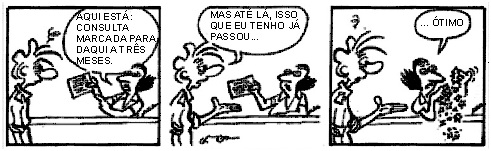
\includegraphics[width=0.5\textwidth]{CIENCIA_DA_COMPUTACAO_Prova2005-utf8_figuras/fig-0002.jpg}
		\caption{Laerte. O condomínio.}
	\end{center}
\end{figure}

\begin{figure}[H]
	\begin{center}
		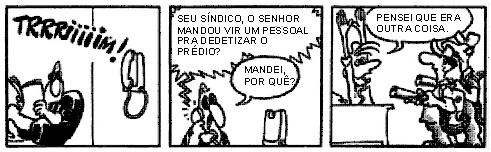
\includegraphics[width=0.5\textwidth]{CIENCIA_DA_COMPUTACAO_Prova2005-utf8_figuras/fig-0003.jpg}
		\caption{Laerte. O condomínio.}
	\end{center}
\end{figure}

As duas charges de Laerte são críticas a dois problemas atuais da sociedade brasileira, que podem ser identificados
	\begin{enumerate}[label=\alph*)]
		\item  pela crise na saúde e na segurança pública.
		\item  pela crise na assistência social e na habitação.
		\item  pela crise na educação básica e na comunicação.
		\item  pela crise na previdência social e pelo desemprego.
		\item  pela crise nos hospitais e pelas epidemias urbanas.
	\end{enumerate}

\question (\textbf{Enade} $|$ \textbf{CC}-\textbf{2005} $|$ \textbf{Objetiva})
Leia trechos da carta-resposta de um cacique indígena à sugestão, feita pelo governo do estado da Virgínia (EUA), de que uma tribo
de índios enviasse alguns jovens para estudar nas escolas dos brancos.
(...) Nós estamos convencidos, portanto, de que os senhores desejam o nosso bem e agradecemos de todo o coração. Mas
aqueles que são sábios reconhecem que diferentes nações têm concepções diferentes das coisas e, sendo assim, os senhores não
ficarão ofendidos ao saber que a vossa idéia de educação não é a mesma que a nossa. (...) Muitos dos nossos bravos guerreiros
foram formados nas escolas do Norte e aprenderam toda a vossa ciência. Mas, quando eles voltaram para nós, eram maus
corredores, ignorantes da vida da floresta e incapazes de suportar o frio e a fome. Não sabiam caçar o veado, matar o inimigo ou
construir uma cabana e falavam nossa língua muito mal. Eles eram, portanto, inúteis. (...) Ficamos extremamente agradecidos pela
vossa oferta e, embora não possamos aceitá-la, para mostrar a nossa gratidão, concordamos que os nobres senhores de Virgínia
nos enviem alguns de seus jovens, que lhes ensinaremos tudo que sabemos e faremos deles homens.
Carlos Rodrigues Brandão. O que é educação. São Paulo: Brasiliense, 1984.
A relação entre os dois principais temas do texto da carta e a forma de abordagem da educação privilegiada pelo cacique está
representada por:
	\begin{enumerate}[label=\alph*)]
		\item  sabedoria e política / educação difusa.
		\item  identidade e história / educação formal.
		\item  ideologia e filosofia / educação superior.
		\item  ciência e escolaridade / educação técnica.
		\item  educação e cultura / educação assistemática.
	\end{enumerate}

\question (\textbf{Enade} $|$ \textbf{CC}-\textbf{2005} $|$ \textbf{Objetiva})

\begin{figure}[H]
	\begin{center}
		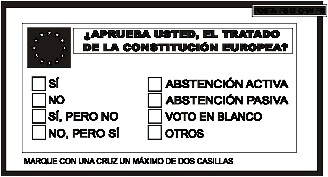
\includegraphics[width=0.5\textwidth]{CIENCIA_DA_COMPUTACAO_Prova2005-utf8_figuras/fig-0005.jpg}
		\caption{La Vanguardia, 4/12/2004}
	\end{center}
\end{figure}

O referendo popular é uma prática democrática que vem sendo
exercida em alguns países, como exemplificado, na charge, pelo
caso espanhol, por ocasião da votação sobre a aprovação ou
não da Constituição Européia. Na charge, pergunta-se com
destaque: “Você aprova o tratado da Constituição Européia?”,
sendo apresentadas várias opções, além de haver a
possibilidade de dupla marcação.
A crítica contida na charge indica que a prática do referendo
deve
	\begin{enumerate}[label=\alph*)]
		\item  ser recomendada nas situações em que o plebiscito já tenha
ocorrido.
		\item  apresentar uma vasta gama de opções para garantir seu
caráter democrático.
		\item  ser precedida de um amplo debate prévio para o
esclarecimento da população.
		\item  significar um tipo de consulta que possa inviabilizar os
rumos políticos de uma nação.
		\item  ser entendida como uma estratégia dos governos para
manter o exercício da soberania.
	\end{enumerate}

\question (\textbf{Enade} $|$ \textbf{CC}-\textbf{2005} $|$ \textbf{Objetiva})

\begin{figure}[H]
	\begin{center}
		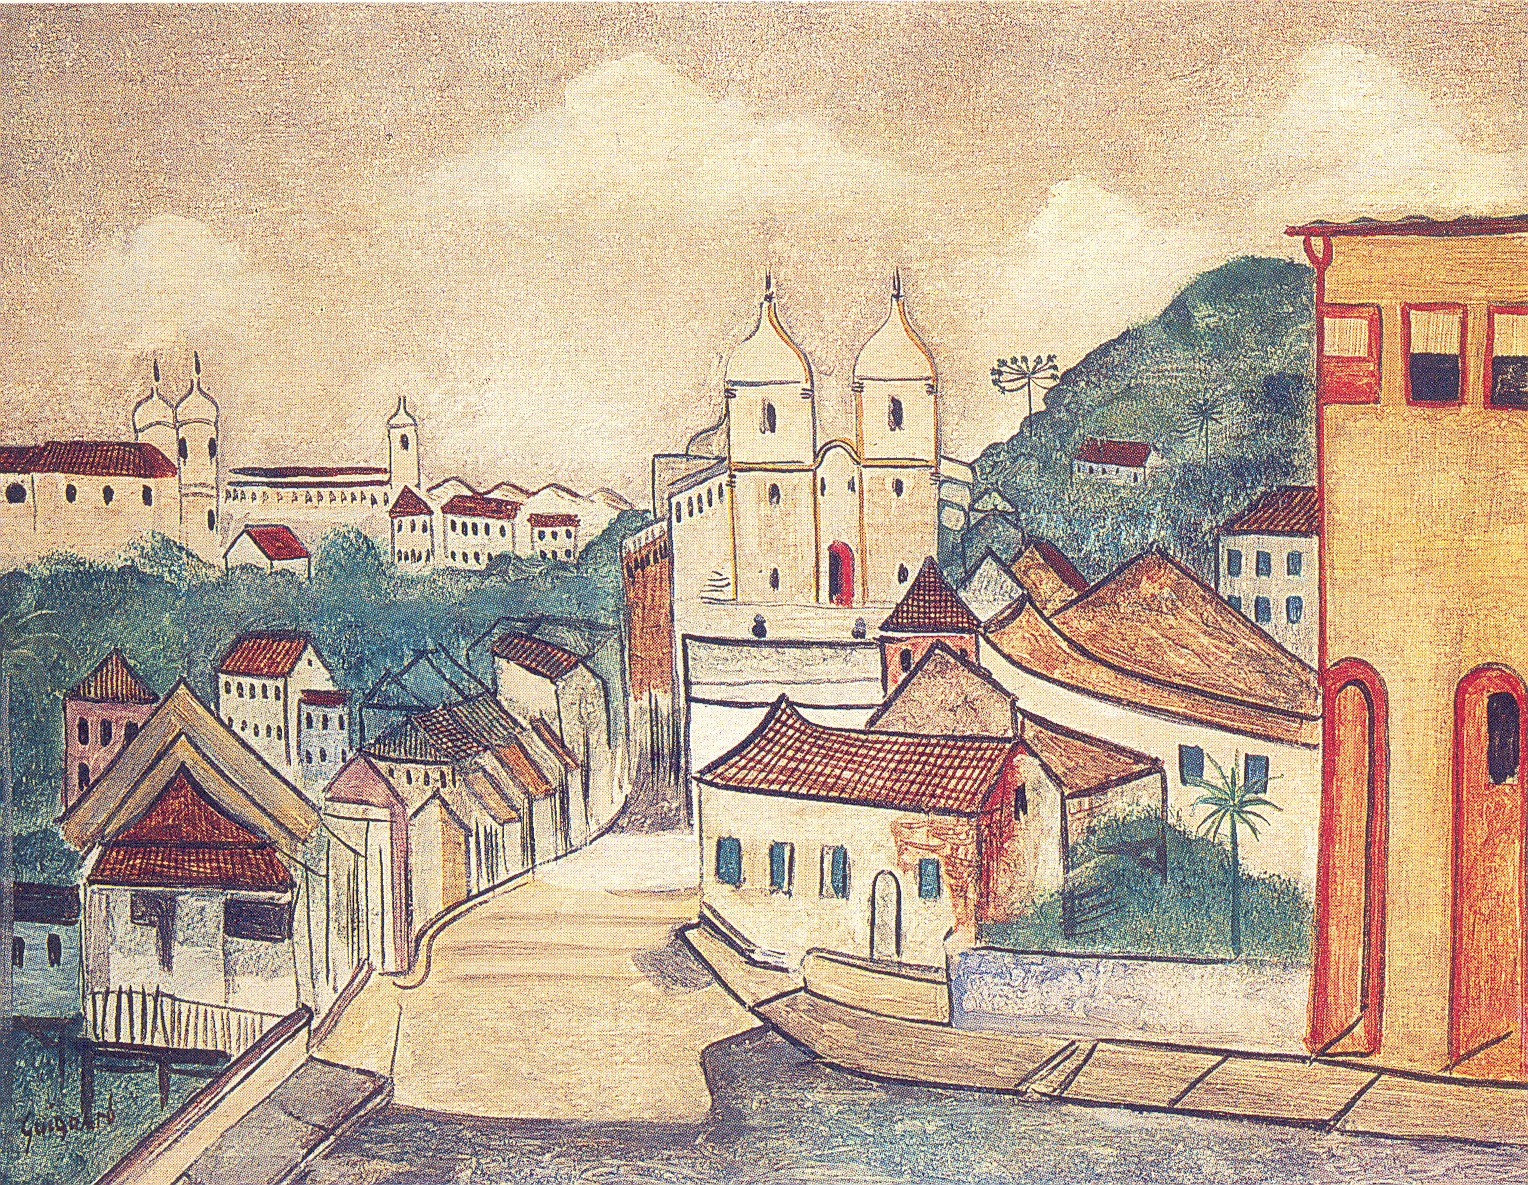
\includegraphics[width=0.5\textwidth]{CIENCIA_DA_COMPUTACAO_Prova2005-utf8_figuras/fig-0004.jpg}
		\caption{Colecção Roberto Marinho. Seis décadas da arte moderna brasileira. Lisboa: Fundação Calouste Gulbenkian, 1989. p. 53}
	\end{center}
\end{figure}

A “cidade” retratada na pintura de Alberto da Veiga Guignard está
tematizada nos versos
	\begin{enumerate}[label=\alph*)]
		\item  Por entre o Beberibe, e o oceano
Em uma areia sáfia, e lagadiça
Jaz o Recife povoação mestiça,
Que o belga edificou ímpio tirano.
Gregório de Matos. Obra poética. Ed. James
Amado. Rio de Janeiro: Record, v. II, 1990. p. 1.191.
		\item  Repousemos na pedra de Ouro Preto,
Repousemos no centro de Ouro Preto:
São Francisco de Assis! igreja ilustre, acolhe,
À tua sombra irmã, meus membros lassos.
Murilo Mendes. Poesia completa e prosa. Org. Luciana
Stegagno Picchio. Rio de Janeiro: Nova Aguilar, 1994, p. 460.
		\item  Bembelelém
Viva Belém!
Belém do Pará porto moderno integrado na equatorial
Beleza eterna da paisagem
Bembelelém
Viva Belém!
Manuel Bandeira. Poesia e prosa. Rio
de Janeiro: Aguilar, v. I, 1958, p. 196.
		\item  Bahia, ao invés de arranhaus, cruzes e cruzes
De braços estendidos para os céus,
E na entrada do porto,
Antes do Farol da Barra,
O primeiro Cristo Redentor do Brasil!
Jorge de Lima. Poesia completa. Org. Alexei
Bueno. Rio de Janeiro: Nova Aguilar, 1997. p. 211.
		\item  No cimento de Brasília se resguardam
maneiras de casa antiga de fazenda,
de copiar, de casa-grande de engenho,
enfim, das casaronas de alma fêmea.
João Cabral Melo Neto. Obra completa. Rio
de Janeiro: Nova Aguilar, 1994, p. 343.
La Vanguardia, 4/12/2004.
JB Ecológico. JB, Ano 4, n.º 41, jun./2005, p.21.
	\end{enumerate}

\question (\textbf{Enade} $|$ \textbf{CC}-\textbf{2005} $|$ \textbf{Dissertativa})

\begin{figure}[H]
	\begin{center}
		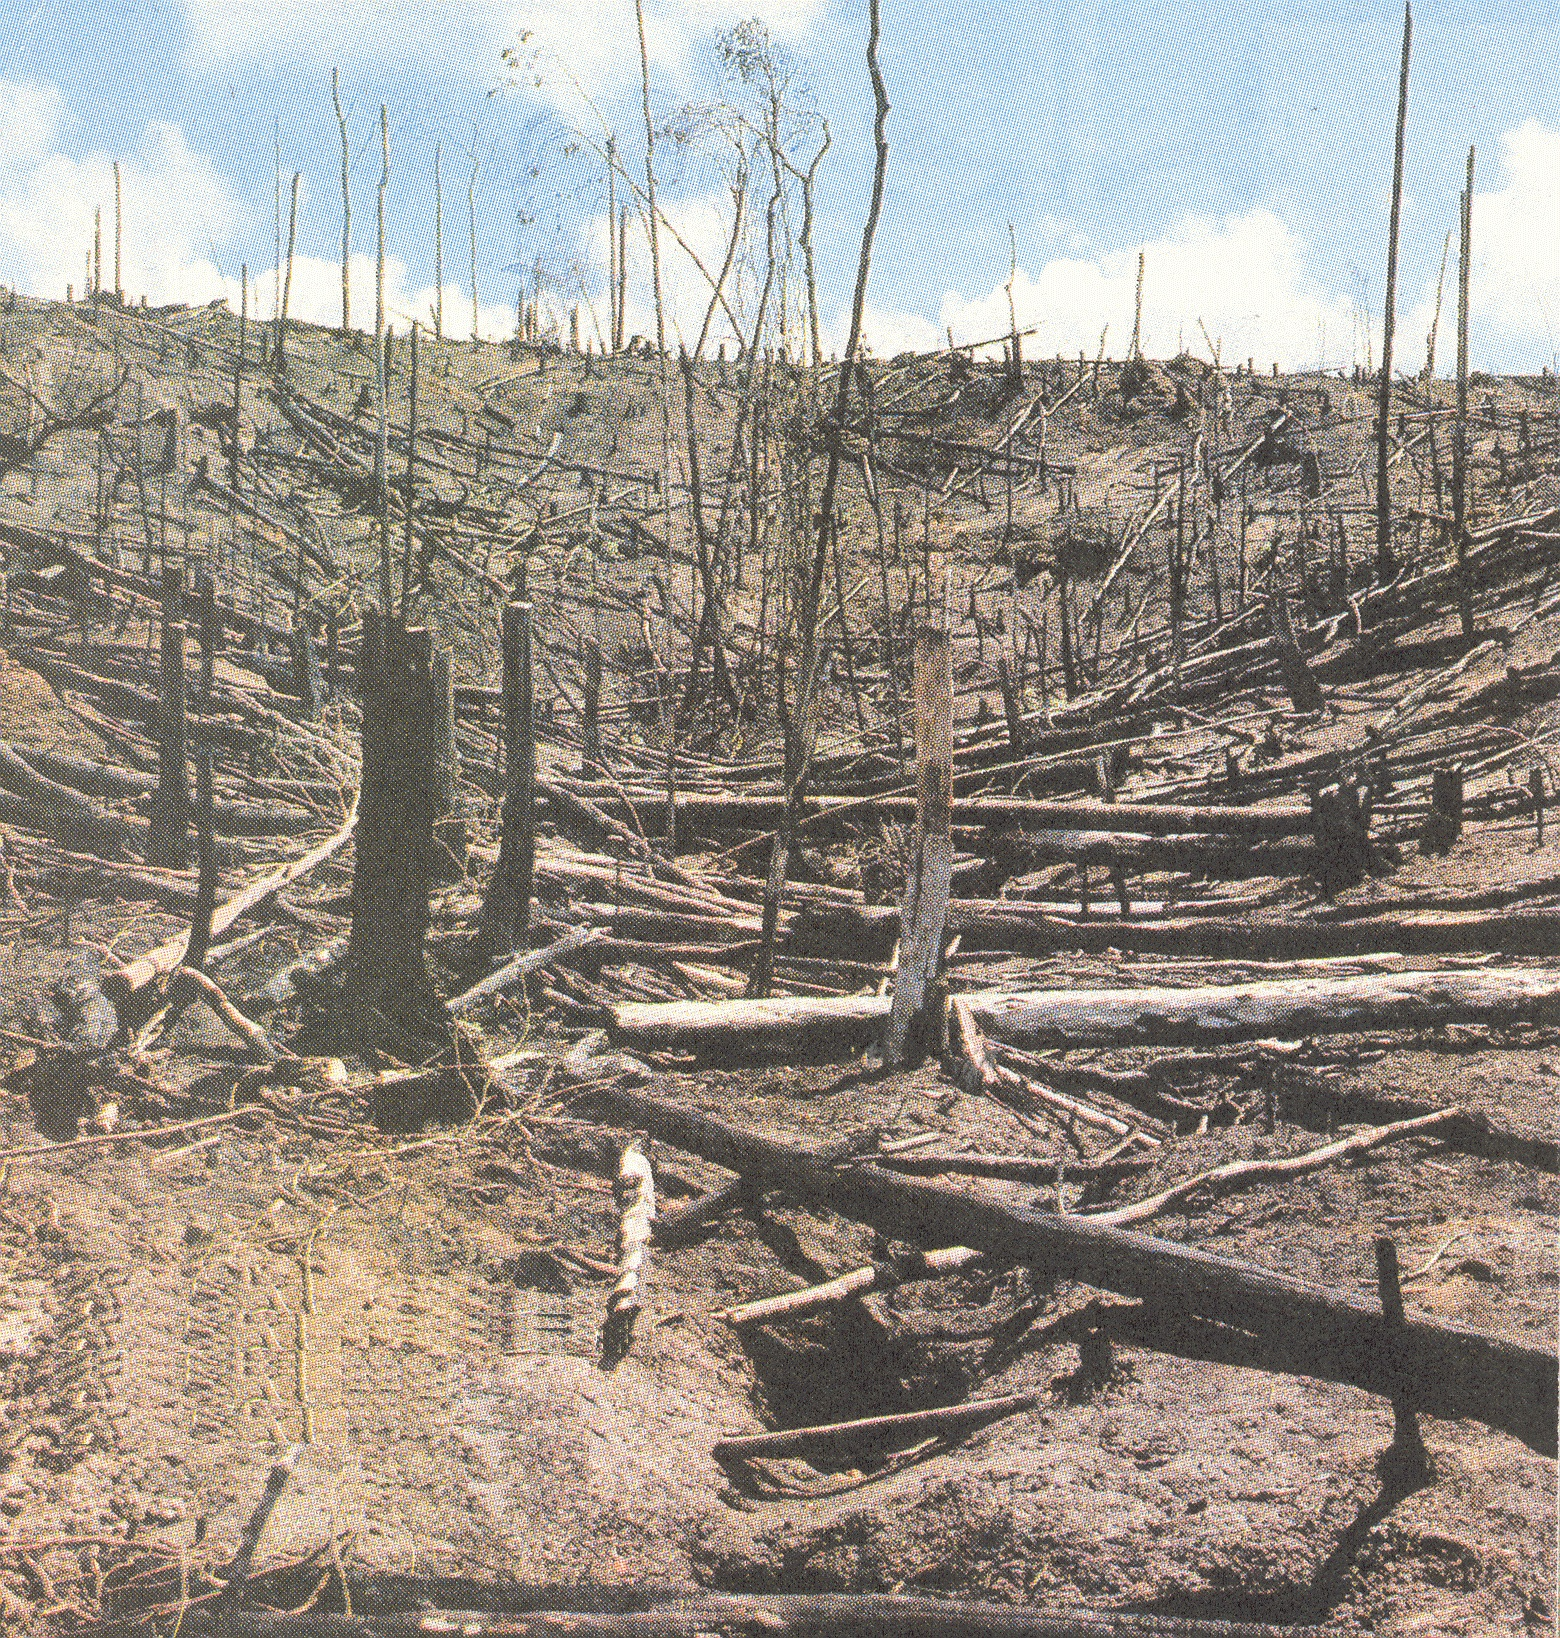
\includegraphics[width=0.5\textwidth]{CIENCIA_DA_COMPUTACAO_Prova2005-utf8_figuras/fig-0006.jpg}
		\caption{JB Ecológico. JB, Ano 4, n.º 41, jun./2005, p.21.}
	\end{center}
\end{figure}

Agora é vero. Deu na imprensa internacional, com base científica
e fotos de satélite: a continuar o ritmo atual da devastação e a
incompetência política secular do Governo e do povo brasileiro em
contê-las, a Amazônia desaparecerá em menos de 200 anos. A última
grande floresta tropical e refrigerador natural do único mundo onde
vivemos irá virar deserto.
Internacionalização já! Ou não seremos mais nada. Nem
brasileiros, nem terráqueos. Apenas uma lembrança vaga e infeliz de vida
breve, vida louca, daqui a dois séculos.
A quem possa interessar e ouvir, assinam essa declaração: todos
os rios, os céus, as plantas, os animais, e os povos índios, caboclos e
universais da Floresta Amazônica. Dia cinco de junho de 2005.
Dia Mundial do Meio Ambiente e Dia Mundial da Esperança. A última.
Felis Concolor. Amazônia? Internacionalização já! In:
JB ecológico. Ano 4, n.º 41, jun./2005, p. 14-5 (com adaptações).
A tese da internacionalização, ainda que circunstancialmente
possa até ser mencionada por pessoas preocupadas com a região, longe está de ser solução para qualquer dos nossos problemas.
Assim, escolher a Amazônia para demonstrar preocupação com o futuro da humanidade é louvável se assumido também, com
todas as suas conseqüências, que o inaceitável processo de destruição das nossas florestas é o mesmo que produz e reproduz
diariamente a pobreza e a desigualdade por todo o mundo.
Se assim não for, e a prevalecer mera motivação “da propriedade”, então seria justificável também propor devaneios
como a internacionalização do Museu do Louvre ou, quem sabe, dos poços de petróleo ou ainda, e neste caso não totalmente
desprovido de razão, do sistema financeiro mundial.
Simão Jatene. Preconceito e pretensão. In: JB ecológico. Ano 4, n.º 42, jul./2005, p. 46-7 (com adaptações).
A partir das idéias presentes nos textos acima, expresse a sua opinião, fundamentada em dois argumentos, sobre
a melhor maneira de se preservar a maior floresta equatorial do planeta.
(valor: 10,0 pontos)
RASCUNHO
1
2
3
4
5
6
7
8
9
10

\question (\textbf{Enade} $|$ \textbf{CC}-\textbf{2005} $|$ \textbf{Dissertativa})
Nos dias atuais, as novas tecnologias se desenvolvem de forma acelerada e a Internet ganha papel importante
na dinâmica do cotidiano das pessoas e da economia mundial. No entanto, as conquistas tecnológicas, ainda que
representem avanços, promovem conseqüências ameaçadoras.
Leia os gráficos e a situação-problema expressa por meio de um diálogo entre uma mulher desempregada, à procura de uma vaga no
mercado de trabalho, e um empregador.
Situação-problema
< mulher:
— Tenho 43 anos, não tenho curso superior
completo, mas tenho certificado de conclusão de
secretariado e de estenografia.
< empregador:
— Qual a abrangência de seu conhecimento sobre o
uso de computadores? Quais as linguagens que
você domina? Você sabe fazer uso da Internet?
< mulher:
— Não sei direito usar o computador. Sou de
família pobre e, como preciso participar
ativamente da despesa familiar, com dois filhos
e uma mãe doente, não sobra dinheiro para
comprar um.
< empregador:
— Muito bem, posso, quando houver uma vaga,
oferecer um trabalho de recepcionista. Para
trabalho imediato, posso oferecer uma vaga de
copeira para servir cafezinho aos funcionários
mais graduados.

\begin{figure}[H]
	\begin{center}
		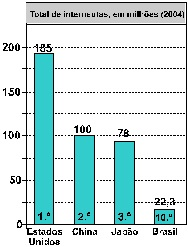
\includegraphics[width=0.5\textwidth]{CIENCIA_DA_COMPUTACAO_Prova2005-utf8_figuras/fig-0007.jpg}
	\end{center}
\end{figure}

\begin{figure}[H]
	\begin{center}
		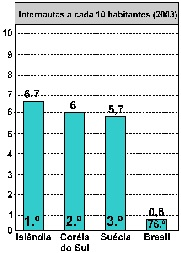
\includegraphics[width=0.5\textwidth]{CIENCIA_DA_COMPUTACAO_Prova2005-utf8_figuras/fig-0008.jpg}
	\end{center}
\end{figure}
Apresente uma conclusão que pode ser extraída da análise
a) dos dois gráficos; (valor: 5,0 pontos)
b) da situação-problema, em relação aos gráficos. (valor: 5,0 pontos)
item a) RASCUNHO
1
2
3
4
5
6
7
8
9
10
Acesso à Internet

item b) RASCUNHO
1
2
3
4
5
6
7
8
9
10
\question (\textbf{Enade} $|$ \textbf{CC}-\textbf{2005} $|$ \textbf{Dissertativa})
Vilarejos que afundam devido ao derretimento da camada congelada do subsolo, uma explosão na
quantidade de insetos, números recorde de incêndios florestais e cada vez menos gelo — esses são alguns dos
sinais mais óbvios e assustadores de que o Alasca está ficando mais quente devido às mudanças climáticas,
disseram cientistas.
As temperaturas atmosféricas no estado norte-americano aumentaram entre 2 C e 3 C nas últimas cinco
o o
décadas, segundo a Avaliação do Impacto do Clima no Ártico, um estudo amplo realizado por pesquisadores
de oito países.
Folha de S. Paulo, 28/9/2005.
O aquecimento global é um fenômeno cada vez mais evidente devido a inúmeros acontecimentos que, como os descritos no texto, têm
afetado toda a humanidade. Apresente duas sugestões de providências a serem tomadas pelos governos que tenham como objetivo
minimizar o processo de aquecimento global. (valor: 10,0 pontos)
RASCUNHO
1
2
3
4
5
6
7
8
9
10

1. As questões de 11 a 40, a seguir, distribuídas de acordo com o quadro abaixo, são
específicas para os estudantes de cursos com perfil de Bacharelado em Sistemas de
Informação. Os demais estudantes deverão passar para a questão de número 41.
PERFIL DO CURSO
NÚMERO DAS QUESTÕES
OBJETIVAS DISCURSIVAS
Bacharelado em Sistemas de Informação 11 a 38 39 e 40
2. Você deve responder apenas às questões referentes ao perfil profissional do curso em que
você está inscrito, de acordo com o estabelecido no cartão de informação do estudante.
3. Favor responder também ao questionário de percepção sobre a prova localizado no final
deste caderno.
As questões de 11 a 40, a seguir, são específicas para os estudantes de cursos com perfil profissional de
BACHARELADO EM SISTEMAS DE INFORMAÇÃO
\question (\textbf{Enade} $|$ \textbf{CC}-\textbf{2005} $|$ \textbf{Objetiva})
Apesar de todo o desenvolvimento, a construção de computadores
e processadores continua, basicamente, seguindo a arquitetura
clássica de von Neumann. As exceções a essa regra encontram-se
em computadores de propósitos específicos e nos desenvolvidos
em centros de pesquisa. Assinale a opção em que estão
corretamente apresentadas características da operação básica de
um processador clássico.
	\begin{enumerate}[label=\alph*)]
		\item  Instruções e dados estão em uma memória física única; um
programa é constituído de uma seqüência de instruções de
máquina; uma instrução é lida da memória de acordo com a
ordem dessa seqüência e, quando é executada, passa-se, então,
para a próxima instrução na seqüência.
		\item  Instruções e dados estão em memórias físicas distintas; um
programa é constituído de um conjunto de instruções de
máquina; uma instrução é lida da memória quando o seu
operando-destino necessita ser recalculado; essa instrução é
executada e o resultado é escrito no operando de destino,
passando-se, então, para o próximo operando a ser recalculado.
		\item  Instruções e dados estão em uma memória física única; um
programa é constituído de um conjunto de instruções de
máquina; uma instrução é lida da memória quando todos os
seus operandos-fonte estiverem prontos e disponíveis; essa
instrução é executada e o resultado é escrito no operando de
destino, passando-se, então, para a instrução seguinte que tiver
todos seus operandos disponíveis.
		\item  Instruções e dados estão em memórias físicas distintas; um
programa é constituído de um conjunto de instruções de
máquina; uma instrução é lida da memória quando todos os
seus operandos-fonte estiverem prontos e disponíveis; essa
instrução é executada e o resultado é escrito no operando de
destino, passando-se, então, para a instrução seguinte que
estiver com todos os seus operandos disponíveis.
		\item  Instruções e dados estão em memórias físicas distintas; um
programa é constituído de uma seqüência de instruções de
máquina; uma instrução é lida da memória de acordo com a
ordem dessa seqüência e, quando é executada, passa-se, então,
para a próxima instrução na seqüência.
	\end{enumerate}

\question (\textbf{Enade} $|$ \textbf{CC}-\textbf{2005} $|$ \textbf{Objetiva})
Um elemento imprescindível em um computador é o sistema de
memória, componente que apresenta grande variedade de tipos,
tecnologias e organizações. Com relação a esse assunto, julgue
os itens seguintes.
I Para endereçar um máximo de 2 palavras distintas, uma
E
memória semicondutora necessita de, no mínimo, E bits de
endereço.
II Em memórias secundárias constituídas por discos
magnéticos, as palavras estão organizadas em blocos, e cada
bloco possui um endereço único, com base na sua
localização física no disco.
III A tecnologia de memória dinâmica indica que o conteúdo
dessa memória pode ser alterado (lido e escrito), ao
contrário da tecnologia de memória estática, cujo conteúdo
pode apenas ser lido, mas não pode ser alterado.
Assinale a opção correta.
	\begin{enumerate}[label=\alph*)]
		\item  Apenas um item está certo.
		\item  Apenas os itens I e II estão certos.
		\item  Apenas os itens I e III estão certos.
		\item  Apenas os itens II e III estão certos.
		\item  Todos os itens estão certos.
	\end{enumerate}

\question (\textbf{Enade} $|$ \textbf{CC}-\textbf{2005} $|$ \textbf{Objetiva})
Julgue os itens a seguir, acerca de algoritmos para ordenação.
I O algoritmo de ordenação por inserção tem complexidade
O(n × log n).
II Um algoritmo de ordenação é dito estável caso ele não altere
a posição relativa de elementos de mesmo valor.
III No algoritmo quicksort, a escolha do elemento pivô
influencia o desempenho do algoritmo.
IV O bubble-sort e o algoritmo de ordenação por inserção
fazem, em média, o mesmo número de comparações.
Estão certos apenas os itens
	\begin{enumerate}[label=\alph*)]
		\item  I e II.
		\item  I e III.
		\item  II e IV.
		\item  I, III e IV.
		\item  II, III e IV.
	\end{enumerate}

\question (\textbf{Enade} $|$ \textbf{CC}-\textbf{2005} $|$ \textbf{Objetiva})
Os proprietários de um teatro necessitam de uma
ferramenta de software para reserva de lugares.
O desenvolvedor contratado verificou que as poltronas
disponíveis para reserva são referenciadas pelo número da fila
(a partir do n. 1) e pelo número da cadeira (a partir do n.
o o
1) em cada fila, em uma representação matricial em que as
linhas e colunas da matriz correspondem, respectivamente, às
filas e às colunas de cadeiras. Embora o contexto seja o da
organização matricial — N filas de cadeiras (linhas), cada uma
contendo M cadeiras (colunas) —, a solução a ser
implementada utilizará uma estrutura linear unidimensional
(vetor), sendo, portanto, necessária uma conversão entre o
lugar referenciado (número f da fila, número c da cadeira) e
a posição real na estrutura de armazenamento (posição p no
vetor).
Na situação apresentada, considere que a referida matriz seja
armazenada no vetor segundo sua seqüência de linhas, da primeira
para a última, e, em cada linha, da primeira coluna para a última,
e que a primeira posição no vetor tenha índice 0. Nessa situação,
a posição p da poltrona do teatro localizada à fila de número f e
à coluna de número c, é igual a
	\begin{enumerate}[label=\alph*)]
		\item  c + f × M.
		\item  f + c × M.
		\item  M × (f – 1) + (c – 1).
		\item  M × (c – 1) + (f – 1).
		\item  M × (c – 1) + M × f.
	\end{enumerate}

\question (\textbf{Enade} $|$ \textbf{CC}-\textbf{2005} $|$ \textbf{Objetiva})
Considere o algoritmo que implementa o seguinte processo: uma
coleção desordenada de elementos é dividida em duas metades e
cada metade é utilizada como argumento para a reaplicação
recursiva do procedimento. Os resultados das duas reaplicações
são, então, combinados pela intercalação dos elementos de ambas,
resultando em uma coleção ordenada. Qual é a complexidade desse
algoritmo?
	\begin{enumerate}[label=\alph*)]
		\item  $O(n^2)$
		\item  $O(n^{2n})$
		\item  $O(2^n)$
		\item  $O(log n × log n)$
		\item  O(n × log n)
	\end{enumerate}

\question (\textbf{Enade} $|$ \textbf{CC}-\textbf{2005} $|$ \textbf{Objetiva})
No processo unificado, cinco workflows acompanham o conjunto
das fases de desenvolvimento de software. Cada workflow é um
conjunto de atividades executadas por vários membros do projeto.
Considerando o desenvolvimento de um sistema integrado de
gestão (ERP), o empacotamento em componentes de software dos
elementos do modelo de projeto — tais como arquivo de código-
fonte, biblioteca de ligação dinâmica e componentes executáveis
— é descrito pelo workflow de
	\begin{enumerate}[label=\alph*)]
		\item  teste.
		\item  análise.
		\item  projeto.
		\item  implementação.
		\item  requisito.
	\end{enumerate}

\question (\textbf{Enade} $|$ \textbf{CC}-\textbf{2005} $|$ \textbf{Objetiva})
No processo de desenvolvimento de um sistema de
controle de materiais (matérias-primas) para uma
metalúrgica, a equipe de projeto, responsável pelo
mapeamento dos requisitos, desenvolveu seus trabalhos
seguindo os quatro subprocessos da engenharia de
requisitos. Inicialmente, foram feitas a análise e a avaliação
para se verificar se o sistema seria útil ao negócio. Em um
segundo momento, os requisitos foram identificados e
analisados e, logo em seguida, foram documentados.
Finalmente, foi verificado se os requisitos identificados
atendiam às demandas dos usuários. Tendo sido executado
esse procedimento, uma empresa independente de
auditoria, após análise, identificou dois problemas no
processo: a documentação dos requisitos (formulários e
padrões utilizados) estava inadequada e não possibilitava
o entendimento correto dos requisitos; o processo de
checagem entre as demandas dos usuários e as
especificações relatadas não foi bem conduzido e seus
resultados eram insatisfatórios.
Considerando o relatório da auditoria independente, quais foram
as duas fases do processo de engenharia de requisitos que
apresentaram problemas?
	\begin{enumerate}[label=\alph*)]
		\item  Entendimento do domínio e especificação.
		\item  Elicitação e validação.
		\item  Validação e entendimento do domínio.
		\item  Especificação e validação.
		\item  Validação e elicitação.
	\end{enumerate}

\question (\textbf{Enade} $|$ \textbf{CC}-\textbf{2005} $|$ \textbf{Objetiva})
No processo de desenvolvimento de um sistema de
tomada de decisões a ser implementado por uma
instituição financeira de natureza privada, um profissional
de sistemas de informações, contratado por prestação de
serviços, recebeu a incumbência de garantir que o novo
sistema operasse com uma função de concessão de crédito
para clientes com maior probabilidade de honrar
compromissos e que representassem menor risco para a
instituição. Para a análise do perfil de cada cliente, o
projetista definiu uma função de pesquisa e cruzamento
de informações obtidas de terceiros e referentes a dados
bancários, pessoais, comerciais, de previdência e saúde, e
gastos com cartão de crédito. Em pouco tempo de
operação, o novo sistema elevou os indicadores de
desempenho da instituição financeira, apesar de ter
diminuído o número de pessoas atendidas com o
programa de concessão de créditos.
Quanto às questões éticas associadas à prática profissional, no
contexto da situação apresentada, julgue os itens abaixo.
I É direito da empresa utilizar qualquer informação
disponível, desde que seja para benefício corporativo.
II A empresa deve controlar, notificar e solicitar
consentimento para armazenar e usar informações dos
clientes.
III A responsabilidade pelo uso correto de informações é de
quem as fornece, de quem as adquire e dos profissionais que
as utilizam na construção de sistemas.
Assinale a opção correta.
	\begin{enumerate}[label=\alph*)]
		\item  Apenas um item está certo.
		\item  Apenas os itens I e II estão certos.
		\item  Apenas os itens I e III estão certos.
		\item  Apenas os itens II e III estão certos.
		\item  Todos os itens estão certos.
	\end{enumerate}

\question (\textbf{Enade} $|$ \textbf{CC}-\textbf{2005} $|$ \textbf{Objetiva})
Julgue os itens seguintes.
I $(\forall x P(x)) \vee (\forall x \neg P(x)) $ é uma sentença válida porque existe
uma interpretação que a torna verdadeira.
II A frase “Se um carro é mais caro que todos os carros
nacionais, ele deve ser alemão” pode ser traduzida pela
seguinte sentença: $\forall x carro(x) \wedge \forall [carro(y) \wedge fabricado(y,Brasil) \wedge (preco(x) > preco(y)) \Rightarrow fabricado(x, Alemanha). $
III A frase “Existe um aluno que gosta de todas as disciplinas
difíceis” pode ser traduzida por: $\exists aluno(x) \wedge \forall y [disciplina(y) \wedge difícil(y)] \wedge gosta(x, y).$
Assinale a opção correta.
	\begin{enumerate}[label=\alph*)]
		\item  Apenas um item está certo.
		\item  Apenas os itens I e II estão certos.
		\item  Apenas os itens I e III estão certos.
		\item  Apenas os itens II e III estão certos.
		\item  Todos os itens estão certos.
	\end{enumerate}

\question (\textbf{Enade} $|$ \textbf{CC}-\textbf{2005} $|$ \textbf{Objetiva})
A orientação a objetos é uma forma abstrata de pensar um
problema utilizando-se conceitos do mundo real e não, apenas,
conceitos computacionais. Nessa perspectiva, a adoção do
paradigma orientado a objetos implica necessariamente que
	\begin{enumerate}[label=\alph*)]
		\item  os usuários utilizem as aplicações de forma mais simples.
		\item  os sistemas sejam encapsulados por outros sistemas.
		\item  os programadores de aplicações sejam mais especializados.
		\item  os objetos sejam implementados de maneira eficiente e
simples.
		\item  a computação seja acionada por troca de mensagens entre
objetos.
	\end{enumerate}

\question (\textbf{Enade} $|$ \textbf{CC}-\textbf{2005} $|$ \textbf{Objetiva})
No modo recursivo de representação, a descrição de um
conceito faz referência ao próprio conceito. Julgue os itens
abaixo, com relação à recursividade como paradigma de
programação.
I São elementos fundamentais de uma definição recursiva:
o caso-base (base da recursão) e a reaplicação da definição.
II O uso da recursão não é possível em linguagens com
estruturas para orientação a objetos.
III As linguagens de programação funcionais têm, na recursão,
seu principal elemento de repetição.
IV No que diz respeito ao poder computacional, as estruturas
iterativas e recursivas são equivalentes.
V Estruturas iterativas e recursivas não podem ser misturadas
em um mesmo programa.
Estão certos apenas os itens
	\begin{enumerate}[label=\alph*)]
		\item  I e IV.
		\item  II e III.
		\item  I, III e IV.
		\item  I, III e V.
		\item  II, IV e V.
	\end{enumerate}

\question (\textbf{Enade} $|$ \textbf{CC}-\textbf{2005} $|$ \textbf{Objetiva})
Com relação ao gerenciamento de memória com paginação em
sistemas operacionais, assinale a opção correta.
	\begin{enumerate}[label=\alph*)]
		\item  As páginas utilizadas por um processo, sejam de código ou de
dados, devem ser obrigatoriamente armazenadas na partição de
swap do disco, quando o processo não estiver sendo executado.
		\item  Todas as páginas de um processo em execução devem ser
mantidas na memória física enquanto o processo não tiver
terminado.
		\item  Um processo somente pode ser iniciado se o sistema
operacional conseguir alocar um bloco contíguo de páginas do
tamanho da memória necessária para execução do processo.
		\item  O espaço de endereçamento virtual disponível para os processos
pode ser maior que a memória física disponível.
		\item  Um processo somente pode ser iniciado se o sistema
operacional conseguir alocar todas as páginas de código
desse processo.
	\end{enumerate}

\question (\textbf{Enade} $|$ \textbf{CC}-\textbf{2005} $|$ \textbf{Objetiva})
Em uma perspectiva instrumental clássica, é possível considerar
que uma organização empresarial esteja dividida em funções e em
níveis hierárquicos ou decisórios. Considere as seguintes
definições.
I Nível responsável pelas decisões mais abrangentes da
organização que possuem impacto no longo prazo e permitem
direcionar e caracterizar o futuro da organização.
II Nível da rotina diária da organização, caracterizado por
decisões de impacto a curto prazo.
III Nível responsável pelas decisões setoriais da organização,
focado na concretização das estratégias a partir do
acompanhamento e do controle das atividades que irão
concretizar os objetivos estabelecidos.
As definições acima correspondem, respectivamente, aos níveis
	\begin{enumerate}[label=\alph*)]
		\item  estratégico, operacional e tático.
		\item  tático, operacional e estratégico.
		\item  operacional, estratégico e tático.
		\item  estratégico, tático e operacional.
		\item  tático, estratégico e operacional.
	\end{enumerate}

\question (\textbf{Enade} $|$ \textbf{CC}-\textbf{2005} $|$ \textbf{Objetiva})
Na definição da aquisição de um novo software de
banco de dados (SGBD) para uma empresa da área de
transporte coletivo urbano, a direção da área de Informática
conduziu o processo de decisão da seguinte forma: foi
designado um profissional da área de banco de dados (aquele
com maior experiência na área) e atribuída a ele a tarefa de
decidir qual seria o melhor SGBD a ser adquirido. Esse
profissional desenvolveu uma série de estudos sobre as opções
disponíveis utilizando técnicas de simulação e testes específicos
para cada SGBD analisado. Ao final, apresentou ao diretor
um relatório em que indicava claramente qual o melhor SGBD
(solução ótima) disponível no mercado. Com base nessa
informação, o diretor da empresa disparou o processo de
compra do software (SGBD) indicado.
Esse processo decisório classifica-se na abordagem
	\begin{enumerate}[label=\alph*)]
		\item  racional.
		\item  de racionalidade limitada.
		\item  política.
		\item  do incrementalismo.
		\item  do componente subjetivo.
	\end{enumerate}

\question (\textbf{Enade} $|$ \textbf{CC}-\textbf{2005} $|$ \textbf{Objetiva})
Entre os aspectos importantes relativos à segurança de sistemas
de informação, inclui-se
I a proteção de dados por meio de senhas e criptografia forte.
II a existência de um plano de recuperação de desastres
associado a backups freqüentes.
III a utilização de firewalls associada a mecanismos de
detecção de intrusão.
Assinale a opção correta.
	\begin{enumerate}[label=\alph*)]
		\item  Apenas um item está certo.
		\item  Apenas os itens I e II estão certos.
		\item  Apenas os itens I e III estão certos.
		\item  Apenas os itens II e III estão certos.
		\item  Todos os itens estão certos.
	\end{enumerate}

\question (\textbf{Enade} $|$ \textbf{CC}-\textbf{2005} $|$ \textbf{Objetiva})
Todo jogador deve pertencer a um único clube.
Assinale a opção que representa corretamente, no modelo
entidade-relacionamento, a especificação apresentada acima.
	\begin{enumerate}[label=\alph*)]
		\item  
\begin{figure}[H]
	\begin{center}
		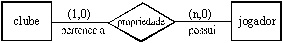
\includegraphics[width=0.5\textwidth]{CIENCIA_DA_COMPUTACAO_Prova2005-utf8_figuras/fig-0010.jpg}
	\end{center}
\end{figure}
		\item  
\begin{figure}[H]
	\begin{center}
		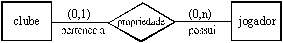
\includegraphics[width=0.5\textwidth]{CIENCIA_DA_COMPUTACAO_Prova2005-utf8_figuras/fig-0011.jpg}
	\end{center}
\end{figure}
		\item  
\begin{figure}[H]
	\begin{center}
		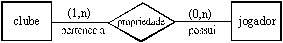
\includegraphics[width=0.5\textwidth]{CIENCIA_DA_COMPUTACAO_Prova2005-utf8_figuras/fig-0012.jpg}
	\end{center}
\end{figure}
		\item  
\begin{figure}[H]
	\begin{center}
		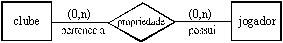
\includegraphics[width=0.5\textwidth]{CIENCIA_DA_COMPUTACAO_Prova2005-utf8_figuras/fig-0013.jpg}
	\end{center}
\end{figure}
		\item  
\begin{figure}[H]
	\begin{center}
		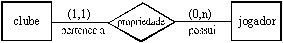
\includegraphics[width=0.5\textwidth]{CIENCIA_DA_COMPUTACAO_Prova2005-utf8_figuras/fig-0014.jpg}
	\end{center}
\end{figure}
	\end{enumerate}

\question (\textbf{Enade} $|$ \textbf{CC}-\textbf{2005} $|$ \textbf{Objetiva})
Na etapa de projeto orientado a objetos, no contexto de um
processo de desenvolvimento de software, são desenvolvidas as
atividades de
	\begin{enumerate}[label=\alph*)]
		\item  definição da arquitetura do sistema e conversão das bases de
dados do sistema.
		\item  identificação dos objetos do sistema e definição da
arquitetura do sistema.
		\item  conversão das bases de dados do sistema e teste de
integração do sistema.
		\item  teste de integração do sistema e análise de requisitos do
sistema.
		\item  análise de requisitos do sistema e definição da arquitetura
do sistema.
	\end{enumerate}

\question (\textbf{Enade} $|$ \textbf{CC}-\textbf{2005} $|$ \textbf{Objetiva})
O gerente de tecnologia de uma empresa de TI
recebeu a incumbência de especificar a arquitetura de um
sistema de informação para atender a um cliente na área de
diagnóstico por imagem (raio X, tomografia computadorizada
e ressonância magnética). O cliente está interessado em
agilizar o diagnóstico por armazenamento e recuperação de
imagens digitalizadas e em se manter na vanguarda do
mercado, dada a melhoria contínua de sua solução em TI.
O cliente pretende iniciar digitalizando 1.000 imagens por
mês, cada imagem com tamanho médio de 20 kilobytes, até
chegar, em 12 meses, a 20.000 imagens por mês.
Considerando essas informações, julgue os seguintes itens.
I Um SBD orientado a objeto é adequado para a arquitetura do SI
do cliente porque é voltado justamente para aplicações que
tratam objetos complexos e tem alta integração com linguagens
de programação orientadas a objetos.
II Um SBD relacional não é adequado para a arquitetura do SI do
cliente porque não constitui ainda uma tecnologia bem
estabelecida e bem testada, apesar de ser uma linguagem de
consulta poderosa.
III Um SBD objeto-relacional é adequado para a arquitetura do SI
do cliente porque alia estruturas não-normalizadas, capazes de
representar objetos complexos, a uma linguagem de consulta
poderosa.
Assinale a opção correta.
	\begin{enumerate}[label=\alph*)]
		\item  Apenas um item está certo.
		\item  Apenas os itens I e II estão certos.
		\item  Apenas os itens I e III estão certos.
		\item  Apenas os itens II e III estão certos.
		\item  Todos os itens estão certos.
	\end{enumerate}

\question (\textbf{Enade} $|$ \textbf{CC}-\textbf{2005} $|$ \textbf{Objetiva})
T1
1 Leitura(X);
2 X = X – 100;
3 Escrita(X);
4 Leitura(Y);
5 Y = Y + 100;
6 Escrita(Y);
Considere um sistema bancário simplificado e uma transação T1,
que transfira R\$ 100,00 da conta X para a conta Y e é definida
pelas operações listadas acima. Considere ainda que uma transação
T2 esteja sendo executada simultaneamente com T1. Caso a
transação T2 realize a operação Escrita(Y) depois da execução
da operação 4 e antes da execução da operação 6 por T1, qual
propriedade de transações será violada no banco de dados do
referido sistema bancário?
	\begin{enumerate}[label=\alph*)]
		\item  Atomicidade.
		\item  Isolamento.
		\item  Distributividade.
		\item  Consistência.
		\item  Durabilidade.
	\end{enumerate}

\question (\textbf{Enade} $|$ \textbf{CC}-\textbf{2005} $|$ \textbf{Objetiva})
O desenvolvimento global de software GSD — global
software development — tem-se firmado como uma das
grandes tendências na área de sistemas de informação nas
organizações. Considere que uma organização da área de
varejo e distribuição sediada na Europa tenha implantado três
unidades de desenvolvimento de software espalhadas no
mundo: uma no Brasil, uma na Índia e outra na China.
Considere ainda que nenhuma dessas unidades possua
qualquer tipo de certificação e que o principal problema da
organização esteja relacionado ao desenvolvimento de
sistemas que atendam às necessidades da organização e que
reflitam as expectativas dos clientes globais.
Nessa situação, o nível do modelo SW-CMM e a KPA (área chave
de processo) mais adequados para a situação apresentada são,
respectivamente,
	\begin{enumerate}[label=\alph*)]
		\item  nível 2, KPA RM – gestão de requisitos.
		\item  nível 2, KPA SPP – planejamento.
		\item  nível 2, KPA SPTO – acompanhamento de projeto.
		\item  nível 3, KPA OPD – definição do processo da organização.
		\item  nível 3, KPA SPE – engenharia de produtos de software.
	\end{enumerate}

\question (\textbf{Enade} $|$ \textbf{CC}-\textbf{2005} $|$ \textbf{Objetiva})
O modelo de gerenciamento de projetos do PMI
(Project Management Institute), descrito no PMBOK, envolve
um conjunto de nove áreas de conhecimento a serem
consideradas com vistas a melhorar o processo de gestão de
um projeto, ampliando-se, conseqüentemente, suas chances
de sucesso. Considere que, no desenvolvimento de um
sistema de vendas de uma empresa que atua no segmento
industrial, o orçamento inicial tenha sido extrapolado em
120% e que a equipe da área de sistemas tenha concluído o
sistema com mais de quatro meses de atraso. Nas reuniões
com os usuários para a entrega do sistema, foi constatado que
este não atendia às especificações esperadas pelos usuários.
Nessa situação, evidenciam-se áreas de conhecimento que
compõem a chamada tripla restrição, que são as áreas de
gerenciamento de
	\begin{enumerate}[label=\alph*)]
		\item  escopo, contratação e custo.
		\item  tempo, contratação e risco.
		\item  custo, tempo e escopo.
		\item  contratação, custo e tempo.
		\item  risco, tempo e escopo.
	\end{enumerate}

\question (\textbf{Enade} $|$ \textbf{CC}-\textbf{2005} $|$ \textbf{Objetiva})
O planejamento estratégico de sistemas de informação pode ser
entendido como o processo de identificação de um porta-fólio
computadorizado de aplicações que dá suporte ao plano de
negócios das organizações e auxilia na concretização dos objetivos
organizacionais. Os principais objetivos do processo de
planejamento estratégico de sistemas de informação não incluem
	\begin{enumerate}[label=\alph*)]
		\item  o alinhamento das estratégias da área de SI com as estratégias
do negócio.
		\item  o comprometimento da alta administração, pela alocação dos
recursos e resultados intermediários e incrementais.
		\item  a melhoria do desempenho da área de SI, seja pela alocação
mais eficaz de recursos, seja pelo aumento de produtividade
dos profissionais.
		\item  a antecipação de tendências, envolvendo inovação tecnológica
contínua.
		\item  a identificação, a avaliação e a validação dos controles
relacionados aos sistemas de informação existentes, do ponto
de vista de sua eficiência e eficácia.
	\end{enumerate}

\question (\textbf{Enade} $|$ \textbf{CC}-\textbf{2005} $|$ \textbf{Objetiva})
Considere que a rede de uma empresa usará os protocolos
TCP/IP para facilitar o acesso do público às informações dessa
empresa a partir de máquinas conectadas à Internet. Considere
ainda que, ao serem descritos os protocolos que serão usados na
rede, alguns erros foram cometidos. As descrições estão
apresentadas nos itens a seguir.
I O Internet Protocol (IP) provê serviço não-orientado a
conexão, e garante a entrega dos datagramas enviados. Além
de garantir a entrega dos datagramas enviados, outra
importante responsabilidade do IP é rotear os datagramas
por meio de redes interligadas. O roteamento é feito usando-
se endereços IP.
II O Internet Control Message Protocol (ICMP) possibilita
que mensagens de erro e de controle sejam trocadas entre
máquinas. As mensagens ICMP são transferidas como dados
em datagramas do IP.
III O Transmission Control Protocol (TCP) provê um serviço
orientado a conexão. Os dados são transferidos por meio de
uma conexão em unidades conhecidas como segmentos.
O TCP espera que a recepção dos segmentos transmitidos
seja confirmada pelo destino e retransmite segmentos cuja
recepção não seja confirmada.
IV O User Datagram Protocol (UDP) provê um mecanismo
para que aplicações possam comunicar-se usando
datagramas. O UDP provê um protocolo de transporte
orientado a conexão e não garante a entrega dos datagramas.
V A emulação de terminal usará o protocolo TELNET, e a
transferência de arquivos, o File Transfer Protocol (FTP).
O correio eletrônico será provido pelo Simple Mail Transfer
Protocol (SMTP) e as mensagens serão transferidas dos
servidores de correio eletrônico para as máquinas dos
usuários via Internet Mail Access Protocol (IMAP).
Estão corretas apenas as descrições
	\begin{enumerate}[label=\alph*)]
		\item  I, II e IV. 
		\item  I, II e V. 
		\item  I, III e IV.
		\item  II, III e V.
		\item  III, IV e V.
	\end{enumerate}

\question (\textbf{Enade} $|$ \textbf{CC}-\textbf{2005} $|$ \textbf{Objetiva})
Julgue os seguintes itens referentes a teste de software.
I A técnica de teste funcional, que estabelece os requisitos de
teste com base em determinada implementação, permite
verificar se são atendidos os detalhes do código e solicita a
execução de partes ou de componentes elementares do
programa; a técnica de teste estrutural aborda o software de
um ponto de vista macroscópico e estabelece os requisitos
de teste, com base em determinada implementação.
II Na fase de teste de unidade, o objetivo é explorar-se a
menor unidade de projeto, procurando-se identificar erros de
lógica e de implementação de cada módulo; na fase de teste
de integração, o objetivo é descobrir erros associados às
interfaces entre os módulos quando esses são integrados,
para se construir a estrutura do software, estabelecida na
fase de projeto.
III Critérios com base na complexidade, em fluxo de controle
e em fluxo de dados, são utilizados pela técnica estrutural de
teste.
Assinale a opção correta.
	\begin{enumerate}[label=\alph*)]
		\item  Apenas um item está certo.
		\item  Apenas os itens I e II estão certos.
		\item  Apenas os itens I e III estão certos.
		\item  Apenas os itens II e III estão certos.
		\item  Todos os itens estão certos.
	\end{enumerate}

\question (\textbf{Enade} $|$ \textbf{CC}-\textbf{2005} $|$ \textbf{Objetiva})
Uma empresa tem a sua sede em Natal e filiais em Brasília e
Florianópolis. Em cada cidade, a empresa possui computadores que
serão interligados. A seguir, encontram-se os requisitos que devem
ser observados no projeto da rede.
Requisito A: Em Natal, existem dois prédios. Para interligá-los,
devem ser usados dispositivos que dividam o tráfego entre os prédios.
Os dispositivos devem atuar na camada de enlace e a presença dos
mesmos deve ser transparente às máquinas na rede.
Requisito B: Em Brasília, há computadores em vários departamentos.
Para interligar os departamentos, devem ser usados dispositivos que
dividam o tráfego entre os departamentos e que possibilitem a
comunicação simultânea entre esses departamentos.
Requisito C: As redes em Natal, Brasília e Florianópolis devem ser
interligadas por dispositivos que dividam o tráfego e que possibilitem
a interligação de redes com diferentes protocolos da camada física.
Para decidir os destinos dos dados, devem ser usados endereços de
rede. Os dispositivos devem possibilitar que o tráfego seja filtrado.
Requisito D: A rede deve usar TCP/IP. O endereço da rede será da
classe B e um dos bytes identificará o segmento da rede localizado em
cada cidade. Em cada segmento, servidores distribuirão
automaticamente os endereços IP entre as máquinas.
Requisito E: Os nomes das máquinas serão traduzidos em endereços
IP por servidores em cada cidade. Esses servidores estarão
organizados em uma hierarquia. Cada servidor será responsável por
um ou por vários subdomínios.
A seguir, encontram-se as decisões que foram tomadas para cada
requisito.
I Usar repetidores para atender ao requisito A.
II Usar comutadores (switches) para atender ao requisito B.
III Usar roteadores para atender ao requisito C.
IV Usar o endereço de rede 164.41.0.0, a máscara 255.255.0.0 e
servidores DHCP para atender ao requisito D.
V Configurar servidores Domain Name System (DNS) para
atender ao requisito E.
Estão corretas apenas as decisões
	\begin{enumerate}[label=\alph*)]
		\item  I, II e IV. 
		\item  I, II e V. 
		\item  I, III e IV.
		\item  II, III e V.
		\item  III, IV e V.
	\end{enumerate}

\question (\textbf{Enade} $|$ \textbf{CC}-\textbf{2005} $|$ \textbf{Objetiva})
João, ao tentar consertar o módulo eletrônico de um
carrinho de brinquedos, levantou as características de um pequeno
circuito digital incluso no módulo. Verificou que o circuito tinha
0 1 0 1
dois bits de entrada, x e x , e um bit de saída. Os bits x e x
eram utilizados para representar valores de inteiros de 0 a 3
0 1
(x , o bit menos significativo e x , o bit mais significativo).
Após testes, João verificou que a saída do circuito é 0 para
todos os valores de entrada, exceto para o valor 2.
Qual das expressões a seguir representa adequadamente o circuito
analisado por João?
0 1
	\begin{enumerate}[label=\alph*)]
		\item  $ x\_0 and (not x\_1 ) $
		\item  $ (not x\_0 ) or (not x\_1 $
		\item  $(not x\_0 ) and x\_1$
		\item  $x\_0 and x\_1$
		\item  $x\_0 or (not x\_1)$
	\end{enumerate}

\question (\textbf{Enade} $|$ \textbf{CC}-\textbf{2005} $|$ \textbf{Objetiva})
O gerente de desenvolvimento de uma empresa de
TI examinou a seguinte planilha sobre andamento de
projetos.
projeto
percentual
completado (em %)
percentual do orçamento
já despendido (em %)
P1 50 70
P2 80 65
Com base nessa planilha e com relação aos conceitos de dado,
informação e conhecimento, julgue os itens que se seguem.
I O número 65, na célula inferior direita, é um dado.
II Associar o número 80 (célula inferior central) ao percentual
completado (em %) e a P2, e concluir que o projeto P2 está
80% completado é um conhecimento.
III Dizer que P1 está adiantado ou atrasado é uma informação.
IV Dizer o quanto P1 vai precisar a mais do que foi
inicialmente previsto no orçamento é um conhecimento.
Estão certos apenas os itens
	\begin{enumerate}[label=\alph*)]
		\item  I e II.
		\item  I e IV.
		\item  II e III.
		\item  II e IV.
		\item  III e IV.
	\end{enumerate}

\question (\textbf{Enade} $|$ \textbf{CC}-\textbf{2005} $|$ \textbf{Objetiva})
O objetivo da Teoria Geral dos Sistemas (TGS) é a formulação
dos princípios válidos para os sistemas em geral, qualquer que
seja a natureza dos elementos que os compõem e as relações ou
forças existentes entre eles. Na área de sistemas de informação,
diversos problemas requerem abordagem multidisciplinar para
serem resolvidos. Por exemplo, na área de desenvolvimento de
software, a especificação de requisitos apresenta vários desafios
desse tipo, tais como aspectos de relacionamento interpessoal,
conhecimento do negócio, resolução de conflitos, diferenças
culturais etc. Os propósitos da TGS que podem contribuir para
a resolução desses problemas incluem
I o incentivo à especialização total das áreas do
conhecimento.
II o desenvolvimento dos princípios unificadores que
transcendem o universo das ciências individuais.
III a integração de contribuições de várias ciências na busca de
solução dos problemas.
IV o desenvolvimento de princípios únicos para cada área do
conhecimento.
V o desenvolvimento de estudos que visem à ampliação da
separação entre as ciências naturais e sociais.
Estão certos apenas os itens
	\begin{enumerate}[label=\alph*)]
		\item  I e II.
		\item  I e V.
		\item  II e III.
		\item  III e IV.
		\item  IV e V.
	\end{enumerate}

\question (\textbf{Enade} $|$ \textbf{CC}-\textbf{2005} $|$ \textbf{Dissertativa})

\begin{figure}[H]
	\begin{center}
		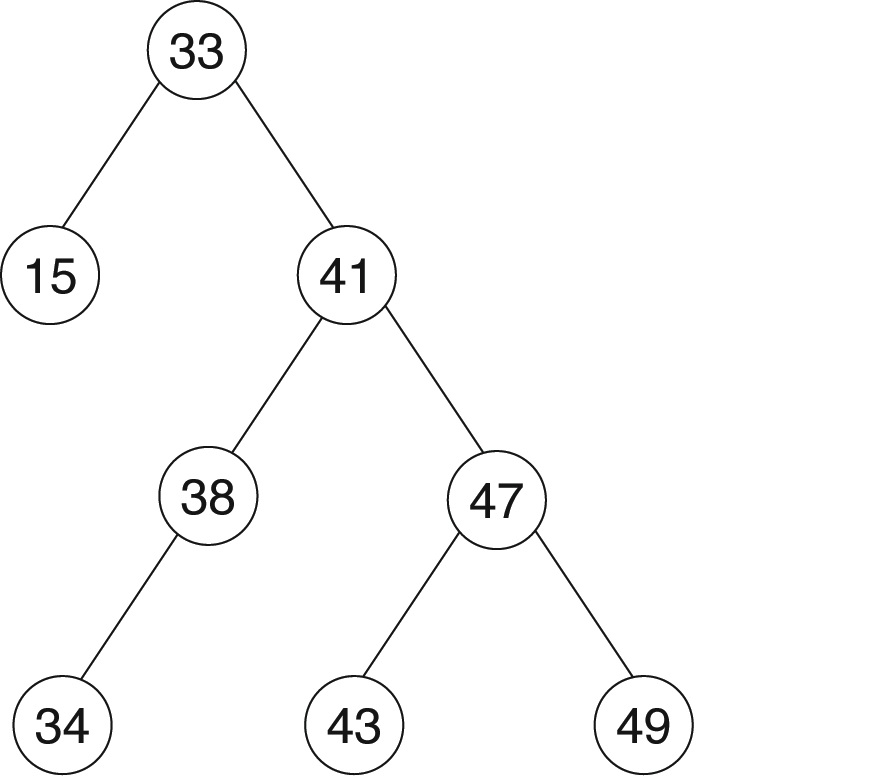
\includegraphics[width=0.5\textwidth]{CIENCIA_DA_COMPUTACAO_Prova2005-utf8_figuras/fig-0015.jpg}
	\end{center}
\end{figure}
Tendo como base a árvore acima, faça o que se pede nos itens a seguir.
a) Descreva uma ordem de visita dos nós para uma busca em profundidade a partir do nó de valor 41. (valor: 3,0 pontos)
b) Considerando que o nó de valor 33 seja a raiz da árvore, descreva a ordem de visita para uma varredura em pré-ordem
(r-e-d, ou pré-fixado à esquerda) na árvore. (valor: 3,0 pontos)
c) Considerando que a árvore cuja raiz é o nó de valor 33 represente uma árvore de busca binária, desenhe a nova árvore que será
obtida após a realização das seguintes operações: inserir um nó de valor 21; remover o nó de valor 47; inserir um nó de valor 48.
(valor: 4,0 pontos)
item a) RASCUNHO
item b) RASCUNHO
item c) RASCUNHO

\question (\textbf{Enade} $|$ \textbf{CC}-\textbf{2005} $|$ \textbf{Dissertativa})
Considere um sistema de locação de filmes em que um cliente solicita a locação de alguns filmes em DVD e após ter-se
identificado ao funcionário e escolhido os filmes, ele os leva para casa, sabendo dos prazos de devolução de cada filme e do
valor do aluguel a ser pago.
Com relação a essa situação,
a) desenhe o diagrama de Caso de Uso correspondente à situação apresentada. (valor: 2,0 pontos)
b) descreva o Caso de Uso relativamente a: atores, pré-condições, pós-condições e fluxo principal. (valor: 5,0 pontos)
c) descreva os tratamentos de exceção do Caso de Uso, considerando duas exceções: cliente em débito (quitação do débito) e filme
reservado para outro cliente (filme não pode ser alugado ao cliente). (valor: 3,0 pontos)
item a) RASCUNHO
item b) RASCUNHO
1
2
3
4
5
6
7
8
9
10
item c) RASCUNHO
1
2
3
4
5
6
7
8
9
10

1. A seguir são apresentadas questões objetivas e discursivas distribuídas do seguinte modo:
PERFIL DO CURSO
NÚMERO DAS QUESTÕES
OBJETIVAS DISCURSIVAS
Bacharelado em Ciência da Computação e
Engenharia de Computação
41 a 54 55
Bacharelado em Ciência da Computação 56 a 69 70
Engenharia de Computação 71 a 84 85
2. Você deve responder apenas às questões referentes ao perfil profissional do curso em que
você está inscrito, de acordo com o estabelecido no cartão de informação do estudante.
3. Favor responder também ao questionário de percepção sobre a prova localizado no final
deste caderno.
As questões de 41 a 55, a seguir, são comuns para os estudantes de cursos com perfil profissional de
BACHARELADO EM CIÊNCIA DA COMPUTAÇÃO e ENGENHARIA DA COMPUTAÇÃO
\question (\textbf{Enade} $|$ \textbf{CC}-\textbf{2005} $|$ \textbf{Objetiva})
Processadores atuais incluem mecanismos para o tratamento
de situações especiais, conhecidas como interrupções. Em uma
interrupção, o fluxo normal de instruções é interrompido para
que a causa da interrupção seja tratada. Com relação a esse
assunto, assinale a opção correta.
	\begin{enumerate}[label=\alph*)]
		\item  Controladores de entrada e saída geram interrupções de
forma síncrona à execução do processador, para que
nenhuma instrução fique incompleta devido à ocorrência
da interrupção.
		\item  Quando uma interrupção ocorre, o próprio processador
salva todo o seu contexto atual, tais como registradores de
dados e endereço e códigos de condição, para que esse
mesmo contexto possa ser restaurado pela rotina de
atendimento da interrupção.
		\item  O processador pode auto-interromper-se para tratar
exceções de execução, tais como um erro em uma
operação aritmética, uma tentativa de execução de
instrução ilegal ou uma falha de página em memória
virtual.
		\item  Rotinas de tratamento de interrupção devem ser executadas
com o mecanismo de interrupção inibido, pois esse tipo de
rotina não permite aninhamento.
		\item  O uso de interrupção para realizar entrada ou saída de
dados somente é eficiente quando o periférico trata
grandes quantidades de dados, como é o caso de discos
magnéticos e discos ópticos. Para periféricos com pouco
volume de dados, como teclados e mouses, o uso de
interrupção é ineficiente.
	\end{enumerate}

\question (\textbf{Enade} $|$ \textbf{CC}-\textbf{2005} $|$ \textbf{Objetiva})
Duas possibilidades para a construção de sistemas com múltiplos
processadores são: processadores idênticos com um único espaço de
endereçamento interligados por um barramento único (SMP); e
máquinas monoprocessadas conectadas por uma rede (cluster). Com
relação a esses sistemas, assinale a opção correta.
	\begin{enumerate}[label=\alph*)]
		\item  comunicação entre processadores de um cluster é,
potencialmente, muito mais rápida que a comunicação entre
processadores de um sistema SMP, pois redes atuais possuem
taxa de transmissão da ordem de gigabits/s, enquanto as
melhores memórias operam somente com freqüências da ordem
de centenas de megahertz.
		\item  Comunicação entre processos pode ser implementada de forma
muito mais eficiente em um cluster que em um sistema SMP,
pois, nesse último, todos os processos precisam compartilhar os
mesmos dispositivos de entrada e saída.
		\item  Em um sistema SMP, é mais simples substituir um processador
defeituoso, pois, em um cluster, toda a rede de comunicação
deve ser desabilitada para que a troca seja efetuada sem
prejudicar a troca de mensagens entre os processos.
		\item  Alocação de memória para processos é muito mais simples em
um cluster, pois cada processador executa um único processo na
sua memória exclusiva e, dessa forma, não existe o problema de
distribuição de processos no espaço de endereçamento único da
máquina SMP.
		\item  Em um cluster, o custo da escalabilidade é muito menor, pois,
para a interconexão entre as máquinas, podem ser utilizados
equipamentos comuns usados em uma rede local de
computadores, ao passo que um sistema SMP exige conexões
extras no barramento e gabinetes especiais.
	\end{enumerate}

\question (\textbf{Enade} $|$ \textbf{CC}-\textbf{2005} $|$ \textbf{Objetiva})
No processo de pesquisa binária em um vetor ordenado, os
números máximos de comparações necessárias para se
determinar se um elemento faz parte de vetores com tamanhos
50, 1.000 e 300 são, respectivamente, iguais a
	\begin{enumerate}[label=\alph*)]
		\item  5, 100 e 30.
		\item  6, 10 e 9.
		\item  8, 31 e 18.
		\item  10, 100 e 30.
		\item  25, 500 e 150.
	\end{enumerate}

\question (\textbf{Enade} $|$ \textbf{CC}-\textbf{2005} $|$ \textbf{Objetiva})
Deseja-se supervisionar as redes de comunicação
de dados de um conjunto de empresas. Cada empresa
tem a sua própria rede, que é independente das redes
das outras empresas e é constituída de ramos de fibra
óptica. Cada ramo conecta duas filiais distintas (ponto-a-
ponto) da empresa. Há, no máximo, um ramo de fibra
interligando diretamente um mesmo par de filiais.
A comunicação entre duas filiais pode ser feita
diretamente por um ramo de fibra que as interliga, se
este existir, ou, indiretamente, por meio de uma
seqüência de ramos e filiais. A rede de cada empresa
permite a comunicação entre todas as suas filiais.
A tabela abaixo apresenta algumas informações acerca
das redes dessas empresas.
empresa n.º de filiais
número de ramos
de fibra entre filiais
E1 9 18
E2 10 45
E3 14 13
E4 8 24
Com relação à situação apresentada acima, é correto deduzir
que,
I no caso da empresa E1, a falha de um ramo de rede
certamente fará que, ao menos, uma filial não possa mais
comunicar-se diretamente com todas as outras filiais da
empresa.
II na rede da empresa E2, a introdução de um novo ramo de
rede certamente violará a informação de que há somente
um par de fibras entre duas filiais.
III no caso da empresa E3, a falha de um único ramo de rede
certamente fará que, ao menos, uma filial não possa mais
comunicar-se, direta ou indiretamente, com todas as outras
filiais da empresa.
IV na rede da empresa E4, todas as filiais da empresa
comunicam-se entre si diretamente.
Estão certos apenas os itens
	\begin{enumerate}[label=\alph*)]
		\item  I e II. 
		\item  I e IV. 
		\item  II e III.
		\item  II e IV.
		\item  III e IV.
	\end{enumerate}

\question (\textbf{Enade} $|$ \textbf{CC}-\textbf{2005} $|$ \textbf{Objetiva})
Requisitos de um sistema são freqüentemente classificados como
funcionais, não-funcionais e de domínio. Qual a definição que
melhor descreve requisitos não-funcionais?
	\begin{enumerate}[label=\alph*)]
		\item  São ferramentas automatizadas de apoio ao processo de
desenvolvimento de sistemas.
		\item  São requisitos que descrevem o que o sistema deve fazer, como
deve reagir a determinadas entradas e como deve comportar-se
em situações particulares.
		\item  São requisitos que derivam do domínio da aplicação e que
refletem características e restrições desse domínio.
		\item  São requisitos que não estão diretamente relacionados com as
funções específicas do sistema.
		\item  São requisitos que especificam como deve ser testada uma parte
do sistema, incluindo-se as entradas, os resultados esperados e as
condições sob as quais os testes devem ocorrer.
	\end{enumerate}

\question (\textbf{Enade} $|$ \textbf{CC}-\textbf{2005} $|$ \textbf{Objetiva})
O Processo Unificado (RUP – rational unified process) é um
moderno processo de desenvolvimento de software constituído de
quatro fases. Assinale a opção que apresenta as quatro fases do RUP,
na ordem em que elas devem ser executadas.
	\begin{enumerate}[label=\alph*)]
		\item  concepção, elaboração, construção, teste
		\item  elaboração, transição, concepção, construção
		\item  elaboração, concepção, teste, transição
		\item  elaboração, concepção, transição, construção
		\item  concepção, elaboração, construção, transição
	\end{enumerate}

\question (\textbf{Enade} $|$ \textbf{CC}-\textbf{2005} $|$ \textbf{Objetiva})
Um estudo recente realizado pela Associação Brasileira das
Empresas de Software (ABES) e a Business Software Alliance
(BSA) mostra uma redução na pirataria de software no mundo e no
Brasil, de 1994 a 2002. Com relação a esse assunto, julgue os itens
a seguir.
I A redução da pirataria de software no contexto brasileiro traz
benefícios para a criação de empregos, aumento da arrecadação
de impostos e aumento no faturamento da economia.
II A reprodução de software original ou autorizado para fins de
segurança ou backup é também considerada pirataria de
software.
III As iniciativas antipirataria devem incluir ações de
conscientização, educação e atuação direta sobre os
contraventores.
IV A pirataria de software é uma atividade criminosa, contudo não
há no Brasil, ainda, legislação específica que regulamente essa
questão.
Estão certos apenas os itens
	\begin{enumerate}[label=\alph*)]
		\item  I e II.
		\item  I e III.
		\item  II e III.
		\item  II e IV.
		\item  III e IV.
	\end{enumerate}

\question (\textbf{Enade} $|$ \textbf{CC}-\textbf{2005} $|$ \textbf{Objetiva})

\begin{figure}[H]
	\begin{center}
		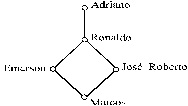
\includegraphics[width=0.5\textwidth]{CIENCIA_DA_COMPUTACAO_Prova2005-utf8_figuras/fig-0017.jpg}
	\end{center}
\end{figure}
Considerando o diagrama de Hasse apresentado acima,
assinale a opção que apresenta uma lista ordenada, da
esquerda para a direita, que preserva a ordem do diagrama.
	\begin{enumerate}[label=\alph*)]
		\item  Marcos, José Roberto, Emerson, Ronaldo, Adriano
		\item  Emerson, Marcos, Ronaldo, Adriano, José Roberto
		\item  Adriano, Ronaldo, José Roberto, Marcos, Emerson
		\item  Ronaldo, Marcos, Emerson, Adriano, José Roberto
		\item  Marcos, Adriano, Emerson, José Roberto, Ronaldo
	\end{enumerate}

\question (\textbf{Enade} $|$ \textbf{CC}-\textbf{2005} $|$ \textbf{Objetiva})
Para o desenvolvimento de um projeto,
determinada organização precisa definir dois grupos de
trabalho, um com três membros e outro com quatro
membros. Para o grupo de três elementos, o primeiro
indivíduo nomeado será o presidente, o segundo, o
relator, e o terceiro será o auxiliar, enquanto que, para
o de quatro elementos, a ordem de nomeação não é
relevante. Essa organização conta com um quadro de
quatorze funcionários, todos igualmente aptos a compor
qualquer um dos grupos de trabalho, em qualquer
função, sendo que cada um deles integrará, no máximo,
um desses grupos.
Nessa situação, representando por C(m, p) a combinação de
m elementos p a p e por A(m, p) o arranjo de m elementos
p a p, conclui-se que a quantidade de maneiras distintas que a
organização citada dispõe para compor os seus dois grupos de
trabalho é igual a
	\begin{enumerate}[label=\alph*)]
		\item  A(14, 4) × A(14, 3).
		\item  A(14, 4) × C(14, 3).
		\item  C(14, 4) × A(10, 3).
		\item  C(10, 3) × A(14, 4).
		\item  C(14, 4) × C(10, 3).
	\end{enumerate}

\question (\textbf{Enade} $|$ \textbf{CC}-\textbf{2005} $|$ \textbf{Objetiva})
Acerca de paradigmas de linguagens de programação, julgue
os itens a seguir.
I Linguagens procedurais facilitam a legibilidade e a
documentação do software.
II Linguagens declarativas facilitam o desenvolvimento de
sistemas de apoio à decisão.
III Linguagens funcionais facilitam a definição de requisitos
e a decomposição funcional.
IV Linguagens estruturadas promovem o forte acoplamento
entre dados e funções.
V Linguagens orientadas a objeto permitem reduzir custos de
desenvolvimento e manutenção.
Estão certos apenas os itens
	\begin{enumerate}[label=\alph*)]
		\item  I e II. 
		\item  I e IV. 
		\item  II e III.
		\item  III e V.
		\item  IV e V.
	\end{enumerate}

\question (\textbf{Enade} $|$ \textbf{CC}-\textbf{2005} $|$ \textbf{Objetiva})

\begin{figure}[H]
	\begin{center}
		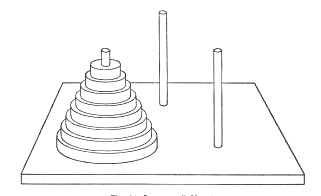
\includegraphics[width=0.5\textwidth]{CIENCIA_DA_COMPUTACAO_Prova2005-utf8_figuras/fig-0018.jpg}
	\end{center}
\end{figure}
No famoso jogo da Torre de Hanoi, é dada uma torre
com discos de raios diferentes, empilhados por tamanho
decrescente em um dos três pinos dados, como ilustra a figura
acima. O objetivo do jogo é transportar-se toda a torre para
um dos outros pinos, de acordo com as seguintes regras:
apenas um disco pode ser deslocado por vez, e, em todo
instante, todos os discos precisam estar em um dos três pinos;
além disso, em nenhum momento, um disco pode ser colocado
sobre um disco de raio menor que o dele; é claro que o
terceiro pino pode ser usado como local temporário para os
discos.
Imaginando que se tenha uma situação em que a torre inicial tenha
um conjunto de 5 discos, qual o número mínimo de movimentações
de discos que deverão ser realizadas para se atingir o objetivo do
jogo?
	\begin{enumerate}[label=\alph*)]
		\item  25
		\item  28
		\item  31
		\item  34
		\item  38
	\end{enumerate}

\question (\textbf{Enade} $|$ \textbf{CC}-\textbf{2005} $|$ \textbf{Objetiva})
O método de alocação de espaço de disco utilizado para
armazenamento de informações em um sistema de arquivos
determina o desempenho desse sistema. Com relação a esse assunto,
julgue os itens seguintes.
I A alocação contígua é um método adequado para sistemas em
que inserções e remoções de arquivos são freqüentes.
II Na alocação indexada, o tamanho máximo de um arquivo
depende do número de bits utilizados para representar um índice
e do tamanho dos blocos de índices.
III Na alocação encadeada, o tamanho máximo de um arquivo
depende do tamanho dos blocos de dados.
Assinale a opção correta.
	\begin{enumerate}[label=\alph*)]
		\item  Apenas um item está certo.
		\item  Apenas os itens I e II estão certos.
		\item  Apenas os itens I e III estão certos.
		\item  Apenas os itens II e III estão certos.
		\item  Todos os itens estão certos.
	\end{enumerate}

\question (\textbf{Enade} $|$ \textbf{CC}-\textbf{2005} $|$ \textbf{Objetiva})
O problema do buffer limitado de tamanho N é um
problema clássico de sincronização de processos: um grupo de
processos utiliza um buffer de tamanho N para armazenar
temporariamente itens produzidos; processos produtores
produzem os itens, um a um, e os armazenam no buffer;
processos consumidores retiram os itens do buffer, um a um,
para processamento. O problema do buffer limitado de tamanho
N pode ser resolvido com a utilização de semáforos, que são
mecanismos de software para controle de concorrência entre
processos. Duas operações são definidas para um semáforo
s: wait(s) e signal(s).
Considere o problema do buffer limitado de tamanho N
cujos pseudocódigos dos processos produtor e consumidor
estão mostrados na tabela abaixo. Pode-se resolver esse
problema com a utilização dos semáforos mutex, cheio e vazio,
inicializados, respectivamente, com 1, 0 e N.
processo produtor processo consumidor
produz item
comando\_a
comando\_b
coloca no buffer
comando\_c
comando\_d
comando\_e
comando\_f
retira do buffer
comando\_g
comando\_h
consome o item
A partir dessas informações, para que o problema do buffer
limitado de tamanho N cujos pseudocódigos foram
apresentados possa ser resolvido a partir do uso dos semáforos
mutex, cheio e vazio, é necessário que comando\_a,
comando\_b, comando\_c, comando\_d, comando\_e,
comando\_f, comando\_g e comando\_h correspondam,
respectivamente, às operações
	\begin{enumerate}[label=\alph*)]
		\item  wait(vazio), wait(mutex), signal(mutex),
signal(cheio), wait(cheio), wait(mutex),
signal(mutex) e signal(vazio).
		\item  wait(cheio), wait(mutex), signal(mutex),
signal(vazio), wait(vazio), signal(mutex),
signal(mutex) e wait(cheio).
		\item  wait(mutex), wait(vazio), signal(cheio),
signal(mutex), wait(mutex), wait(vazio),
signal(cheio) e signal(mutex).
		\item  wait(mutex), wait(vazio), signal(cheio),
signal(mutex), wait(mutex), wait(cheio),
signal(vazio) e signal(mutex).
		\item  wait(vazio), signal(mutex), signal(cheio),
wait(mutex), wait(cheio), signal(mutex),
signal(vazio) e signal(mutex).
	\end{enumerate}

\question (\textbf{Enade} $|$ \textbf{CC}-\textbf{2005} $|$ \textbf{Objetiva})
Considere que, durante a análise de um problema de programação,
tenha sido obtida a seguinte fórmula recursiva que descreve a
solução para o problema.
Qual a complexidade da solução encontrada?
	\begin{enumerate}[label=\alph*)]
		\item  O (n × log n)
		\item  O (n )
2
		\item  O (n × log n)
2
		\item  O (2 )
n
		\item  O (n )
3
RASCUN H O
	\end{enumerate}

\question (\textbf{Enade} $|$ \textbf{CC}-\textbf{2005} $|$ \textbf{Dissertativa})
O grande desejo de todos os desenvolvedores de programas é utilizar quantidades ilimitadas de memória que, por sua vez,
seja extremamente rápida. Infelizmente, isso não corresponde à realidade, como tenta representar a figura abaixo, que descreve
uma hierarquia de memória: para cada elemento, estão indicados os tamanhos típicos disponíveis para armazenamento de
informação e o tempo típico de acesso à informação armazenada.


\begin{figure}[H]
	\begin{center}
		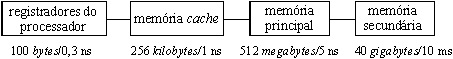
\includegraphics[width=0.5\textwidth]{CIENCIA_DA_COMPUTACAO_Prova2005-utf8_figuras/fig-0019.jpg}
	\end{center}
\end{figure}

Como pode ser visto no diagrama acima, registradores do processador e memória cache operam com tempos distintos, o
mesmo ocorrendo com a memória principal com relação à memória cache, e com a memória secundária com relação à memória
principal.
Considerando as informações acima apresentadas, responda às seguintes perguntas.
a) Que características um programa deve ter para que o uso de memória cache seja muito vantajoso? (valor: 4,0 pontos)
b) Se registradores do processador e a memória cache operassem com os mesmos tempos de acesso, ainda haveria vantagem em se
utilizar a memória cache? E se a memória cache e a memória principal operassem com os mesmos tempos de acesso, ainda haveria
vantagem em se utilizar a memória cache? Justifique suas respostas. (valor: 6,0 pontos)
item a) RASCUNHO
1
2
3
4
5
item b) RASCUNHO
1
2
3
4
5
6
7
8
9
10

As questões de 56 a 70, a seguir, são específicas para os estudantes de cursos com perfil profissional de
BACHARELADO EM CIÊNCIA DA COMPUTAÇÃO
\question (\textbf{Enade} $|$ \textbf{CC}-\textbf{2005} $|$ \textbf{Objetiva})
Considere um sistema bancário
simplificado e uma transação T1,
que, por meio das 6 operações
apresentadas na tabela ao lado,
transfere R\$ 100,00 da conta X
para a conta Y. A partir dessas
informações, julgue os itens que se
seguem.

I Se, durante a execução de T1,
ocorrer uma falha depois da
operação 3 e antes da operação
6, e o sistema de banco de dados
restabelecer o valor original
de X, estará garantida a atomicidade de T1. 

II Se ocorrer uma falha de sistema após a transação T1 ser
completada com sucesso, mas, ao ser reiniciado o sistema, o
usuário que a tiver disparado for notificado da transferência
de fundos e o sistema de banco de dados reconstruir as
atualizações feitas pela transação, estará garantida a
durabilidade de T1. 

III Se outra transação, T2, que estiver sendo executada
simultaneamente a T1, tentar executar a operação
escrita(Y) depois de T1 ter executado a operação 4 e
ainda não ter executado a operação 6, e o sistema de banco
de dados impedir essa escrita, estará garantida a consistência
de T1.

Assinale a opção correta.
	\begin{enumerate}[label=\alph*)]
		\item  Apenas um item está certo.
		\item  Apenas os itens I e II estão certos.
		\item  Apenas os itens I e III estão certos.
		\item  Apenas os itens II e III estão certos.
		\item  Todos os itens estão certos.
	\end{enumerate}

\question (\textbf{Enade} $|$ \textbf{CC}-\textbf{2005} $|$ \textbf{Objetiva})
A escolha de uma boa representação de conhecimento é tarefa
fundamental na resolução de problemas que envolvem
inteligência artificial. Acerca desse assunto, assinale a opção
correta.
	\begin{enumerate}[label=\alph*)]
		\item  O encadeamento regressivo, por utilizar busca em largura
para resolução de conflitos, é menos usado que o progressivo.
		\item  O encadeamento progressivo utiliza busca gulosa para fazer
a comparação entre os fatos armazenados na memória de
trabalho do sistema e os antecedentes das regras a disparar.
		\item  As redes semânticas, mecanismo mais expressivo que a
lógica de primeira ordem, foram desenvolvidas para se
superar uma dificuldade dos sistemas embasados em lógica
de representar categorias.
		\item  A representação de conhecimento frames é uma boa
alternativa para esse tipo de problema, por incluir, além de
um mecanismo de inferência semanticamente bem definido,
mecanismos de encapsulamento e componentes, comuns ao
paradigma orientado a objeto.
		\item  Tanto redes semânticas quanto frames representam
facilmente conhecimento estrutural, comportamental e
procedural.
	\end{enumerate}

\question (\textbf{Enade} $|$ \textbf{CC}-\textbf{2005} $|$ \textbf{Objetiva})

\begin{figure}[H]
	\begin{center}
		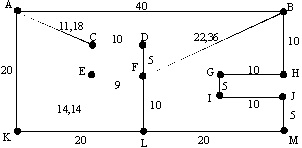
\includegraphics[width=0.5\textwidth]{CIENCIA_DA_COMPUTACAO_Prova2005-utf8_figuras/fig-0020.jpg}
	\end{center}
\end{figure}
Uma forma de analisar e comparar o desempenho de algoritmos
de busca heurística é utilizar um problema bem conhecido como
referência. Um exemplo desse tipo de problema é o cálculo de
rotas entre diferentes cidades. No grafo ilustrado acima, cada nó
representa uma cidade distinta, e cada ramo, uma rodovia que
interliga as cidades representadas pelos nós que ele une, cujo peso
indica a distância, em km, entre essas cidades pela rodovia.
Suponha que se deseje encontrar a melhor rota entre as cidades A
e M, indicadas nesse grafo. Considere, ainda, os valores indicados
na tabela abaixo como distância em linha reta, em km, de cada
cidade para a cidade M.
A 44,72 E 30,67 I 11,18
B 20,00 F 22,36 J 5,00
C 33,54 G 14,14 K 40,00
D 25,00 H 10,00 L 20,00
A partir dessas informações, julgue os itens seguintes, relativos a
algoritmos de busca.
I Utilizando-se o algoritmo A*, a rota ente A e M encontrada no
problema acima é ACDFLM e o custo do caminho é 56,18.
II Utilizando-se a busca gulosa, a rota encontrada no problema
acima é ACDFLM.
III Para utilizar algoritmos de busca heurística, deve-se definir
uma heurística que superestime o custo da solução.
IV O A* é um algoritmo ótimo e completo quando heurísticas
admissíveis são utilizadas.
V No simulated annealing, é possível haver movimentos para um
estado com avaliação pior do que a do estado corrente,
dependendo da temperatura do processo e da probabilidade
de escolha.
Estão certos apenas os itens
	\begin{enumerate}[label=\alph*)]
		\item  I, II e III.
		\item  I, IV e V.
		\item  I, III, e V.
		\item  II, III, e IV.
		\item  II, IV e V.
T1
1 leitura(X);
2 X = X – 100;
3 escrita(X);
4 leitura(Y);
5 Y = Y + 100;
6 escrita (Y);
	\end{enumerate}

\question (\textbf{Enade} $|$ \textbf{CC}-\textbf{2005} $|$ \textbf{Objetiva})
Considere o seguinte esquema relacional para o banco de dados de um grande banco com cobertura nacional.
AGENCIAS(NOME\_AGENCIA, CIDADE\_AGENCIA, FUNDOS);
CONTAS(NOME\_AGENCIA, NUMERO\_CONTA, SALDO) NOME\_AGENCIA REFERENCIA AGENCIAS;
CLIENTES(NOME\_CLIENTE, CIDADE\_NASCIMENTO, NUMERO\_CONTA) NUMERO\_CONTA REFERENCIA CONTAS;
Considere, ainda, que os atributos sublinhados correspondam às chaves primárias das respectivas relações e, após as definições das
relações CONTAS e CLIENTES, sejam descritas as regras de integridade referenciais. Suponha que o banco de dados armazene
informações de 500 agências, de 1.000.000 de contas e de 1.500.000 clientes, sendo que 200.000 contas são de agências da cidade
de São Paulo e 100.000 clientes nasceram em Recife. Considere, finalmente, que esse sistema de banco de dados tenha um otimizador
de consultas embasado em heurísticas e que se precise realizar a seguinte consulta.
SELECT *
FROM AGENCIAS, CONTAS, CLIENTES
WHERE CONTAS.NOME\_AGENCIA = AGENCIAS.NOME\_AGENCIA
AND CLIENTES.NUMERO\_CONTA = CONTAS.NUMERO\_CONTA
AND CIDADE\_AGENCIA = ‘SAO PAULO’
AND CIDADE\_NASCIMENTO = ‘RECIFE’
AND SALDO > 1000;
A partir dessas informações e considerando  o operador de junção natural e F o operador de seleção, assinale a opção que apresenta
\begin{figure}[H]
	\begin{center}
		
\includegraphics[width=0.5\textwidth]{CIENCIA_DA_COMPUTACAO_Prova2005-utf8_figuras/fig-0021.jpg}
	\end{center}
\end{figure}
o melhor plano de avaliação de consultas para a consulta apresentada acima.
	\begin{enumerate}[label=\alph*)]
		\item  
\begin{figure}[H]
	\begin{center}
		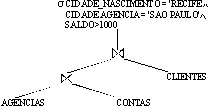
\includegraphics[width=0.5\textwidth]{CIENCIA_DA_COMPUTACAO_Prova2005-utf8_figuras/fig-0022.jpg}
	\end{center}
\end{figure}
		\item 	
\begin{figure}[H]
	\begin{center}
		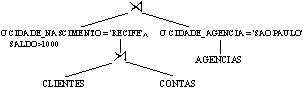
\includegraphics[width=0.5\textwidth]{CIENCIA_DA_COMPUTACAO_Prova2005-utf8_figuras/fig-0023.jpg}
	\end{center}
\end{figure}
		\item 	
\begin{figure}[H]
	\begin{center}
		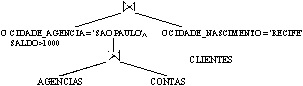
\includegraphics[width=0.5\textwidth]{CIENCIA_DA_COMPUTACAO_Prova2005-utf8_figuras/fig-0024.jpg}
	\end{center}
\end{figure}
		\item 	
\begin{figure}[H]
	\begin{center}
		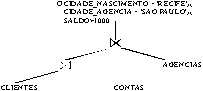
\includegraphics[width=0.5\textwidth]{CIENCIA_DA_COMPUTACAO_Prova2005-utf8_figuras/fig-0025.jpg}
	\end{center}
\end{figure}
		\item 	
\begin{figure}[H]
	\begin{center}
		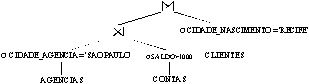
\includegraphics[width=0.5\textwidth]{CIENCIA_DA_COMPUTACAO_Prova2005-utf8_figuras/fig-0026.jpg}
	\end{center}
\end{figure}
	\end{enumerate}

\question (\textbf{Enade} $|$ \textbf{CC}-\textbf{2005} $|$ \textbf{Objetiva})


\begin{figure}[H]
	\begin{center}
		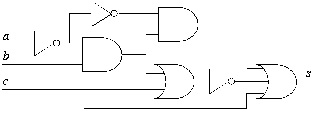
\includegraphics[width=0.5\textwidth]{CIENCIA_DA_COMPUTACAO_Prova2005-utf8_figuras/fig-0029.jpg}
	\end{center}
\end{figure}

Considere o circuito combinacional ilustrado acima, que apresenta
a, b e c como sinais de entrada e s como sinal de saída. A equação
booleana mínima que descreve a função desse circuito é igual a
	\begin{enumerate}[label=\alph*)]
		\item  s = a or not(b) or c.
		\item  s = a and not(b) and c.
		\item  s = not(a) or b or not(c).
		\item  s = not(a) and b and not(c).
		\item  s = (not(a) and b) or c.
	\end{enumerate}

\question (\textbf{Enade} $|$ \textbf{CC}-\textbf{2005} $|$ \textbf{Objetiva})

\begin{figure}[H]
	\begin{center}
		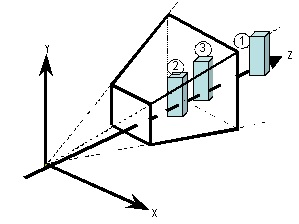
\includegraphics[width=0.5\textwidth]{CIENCIA_DA_COMPUTACAO_Prova2005-utf8_figuras/fig-0030.jpg}
	\end{center}
\end{figure}
Considere o volume de visualização e os objetos identificados
como Î, Ï e Ð na figura acima. Considere, ainda, que todos os
objetos têm o mesmo tamanho, que o objeto Î está localizado fora
do volume de visualização e que os objetos Ï e Ð estão dentro
dele. A partir desses dados, no que concerne à execução do
pipeline de visualização na situação acima representada, é correto
inferir que
I o objeto Î está na linha de visão do observador, mas não
aparece na imagem final.
II é suficiente, para a determinação das faces visíveis, realizar o
recorte contra o volume canônico.
III a remoção de faces traseiras (back face culling) utiliza
informação de posição e orientação do observador.
IV o processo de visualização garante que os objetos Ï e Ð sejam
totalmente visíveis na imagem final.
Estão certos apenas os itens
	\begin{enumerate}[label=\alph*)]
		\item  I e II.
		\item  I e III.
		\item  II e III.
		\item  III e IV.
		\item  III e IV.
	\end{enumerate}

\question (\textbf{Enade} $|$ \textbf{CC}-\textbf{2005} $|$ \textbf{Objetiva})

\begin{figure}[H]
	\begin{center}
		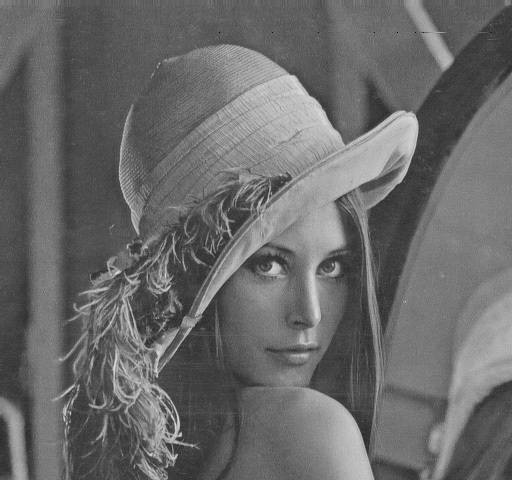
\includegraphics[width=0.5\textwidth]{CIENCIA_DA_COMPUTACAO_Prova2005-utf8_figuras/fig-0027.jpg}
	\end{center}
\end{figure}

\begin{figure}[H]
	\begin{center}
		
\includegraphics[width=0.5\textwidth]{CIENCIA_DA_COMPUTACAO_Prova2005-utf8_figuras/fig-0028.jpg}
		\caption{II}
	\end{center}
\end{figure}
Considere que um colega seu tenha ganhado uma máquina
fotográfica digital e tenha tirado a foto identificada por I acima.
Na seqüência, a partir da imagem I, considere que ele tenha
gerado a imagem II acima. Nessa situação, o processamento
realizado sobre a imagem I que melhor explica a geração da
imagem II envolve a aplicação de
	\begin{enumerate}[label=\alph*)]
		\item  filtro passaixas.
		\item  quantizador.
		\item  reamostragem.
		\item  filtro passatas.
		\item  compressão.
	\end{enumerate}

\question (\textbf{Enade} $|$ \textbf{CC}-\textbf{2005} $|$ \textbf{Objetiva})
estado
símbolo
lido na fita
símbolo gravado
na fita
direção
próximo
estado
início ! ! direita 0
0 0 1 direita 0
0 1 0 direita 0
0 - - esquerda 1
1 0 0 esquerda 1
1 1 1 esquerda 1
1 ! ! direita parada
Na tabela acima, estão descritas as ações correspondentes a cada
um dos quatro estados (início, 0, 1, parada) de uma máquina de
Turing, que começa a operar no estado “início” processando
símbolos do alfabeto {0,1,!, -}, em que ‘-’ representa o espaço
em branco. Considere que, no estado “início”, a fita a ser
processada esteja com a cabeça de leitura/gravação na posição 1,
conforme ilustrado a seguir.
1 2 3 4 5 6 7 8 9 10 11 ...
! 0 1 1 0 1 - - - - - ...
Considerando essa situação, assinale a opção que indica
corretamente a posição da cabeça de leitura/gravação e o conteúdo
da fita após o término da operação, ou seja, após a máquina atingir
o estado “parada”.
	\begin{enumerate}[label=\alph*)]
		\item 
1 2 3 4 5 6 7 8 9 10 11 ...
! 0 0 1 1 1 1 0 0 1 1 ...
		\item 
1 2 3 4 5 6 7 8 9 10 11 ...
! 0 1 1 0 1 - - - - - ...
		\item 
1 2 3 4 5 6 7 8 9 10 11 ...
! 0 1 1 0 1 0 1 0 0 1 ...
		\item 
1 2 3 4 5 6 7 8 9 10 11 ...
! - - - - - 1 - - - - ...
		\item 
1 2 3 4 5 6 7 8 9 10 11 ...
! 1 0 0 1 0 - - - - - ...
	\end{enumerate}

\question (\textbf{Enade} $|$ \textbf{CC}-\textbf{2005} $|$ \textbf{Objetiva})
Considere a necessidade de se implementar um componente de
software que realiza cálculos de expressões matemáticas simples
para as operações básicas (soma, subtração, multiplicação, divisão
e exponenciação). O software reproduz na tela do computador a
entrada, os resultados parciais e o resultado final da expressão e,
ainda, trata os operadores de exponenciação, multiplicação e
divisão com precedência sobre os operadores de soma e subtração.
Para obter o referido software, é correto que o projetista
I defina uma cadeia de caracteres para armazenar e imprimir toda
a expressão de entrada.
II defina uma gramática regular para identificar as expressões
aritméticas válidas.
III defina um reconhecedor de linguagem regular com autômato
finito determinístico.
IV especifique a ordem de precedência dos operadores com uma
notação de gramática livre de contexto.
Estão certos apenas os itens
	\begin{enumerate}[label=\alph*)]
		\item  I e II. 
		\item  III e IV. 
		\item  I, II e IV.
		\item  I, III e IV.
		\item  II, III e IV.
	\end{enumerate}

\question (\textbf{Enade} $|$ \textbf{CC}-\textbf{2005} $|$ \textbf{Objetiva})
A análise de complexidade provê critérios para a classificação
de problemas com base na computabilidade de suas soluções,
utilizando-se a máquina de Turing como modelo referencial e
possibilitando o agrupamento de problemas em classes. Nesse
contexto, julgue os itens a seguir.
I É possível demonstrar que P f NP e NP f P.
II É possível demonstrar que se P … NP, então
P 1 NP-Completo = i.
III Se um problema Q é NP-difícil e Q 0 NP, então Q é
NP-completo.
IV O problema da satisfatibilidade de uma fórmula booleana F
(uma fórmula é satisfatível, se é verdadeira em algum
modelo) foi provado ser NP-difícil e NP-Completo.
V Encontrar o caminho mais curto entre dois vértices dados
em um grafo de N vértices e M arestas não é um problema
da classe P.
Estão certos apenas os itens
	\begin{enumerate}[label=\alph*)]
		\item  I, III e IV.
		\item  II, III, e IV.
		\item  III, IV e V.
		\item  I, II, III, e IV.
		\item  II, III, IV e V.
	\end{enumerate}

\question (\textbf{Enade} $|$ \textbf{CC}-\textbf{2005} $|$ \textbf{Objetiva})
Considere que, em uma empresa que desenvolve aplicações
distribuídas, tenha sido elaborado um manual destinado ao
treinamento de empregados e que o responsável por elaborar o
manual tenha cometido alguns erros. Analise os seguintes
trechos do referido manual.
I Uma aplicação que usa o User Datagram Protocol (UDP)
para transporte dos dados pode ter de tratar os problemas
decorrentes de perdas de mensagens, mensagens recebidas
fora de ordem e duplicações de mensagens.
II Um mecanismo de chamada a procedimento remoto (remote
procedure call) ou de invocação a método remoto (remote
method invocation) possibilita que programas chamem
procedimentos ou métodos em diferentes computadores e
que se abstraiam de todos os detalhes relacionados à
distribuição.
III Em um sistema de comunicação embasado na chamada a
procedimento remoto ou na invocação de método remoto, os
serviços remotos são definidos por meio de interfaces. Uma
interface é tipicamente processada por um compilador que
gera códigos (stubs), que, nos clientes, se fazem passar pelos
códigos remotos que são chamados.
IV Sistemas de chamada a procedimentos remotos ou de
invocação a métodos remotos tipicamente implementam as
semânticas at-most-once ou at-least-once, pois é mais difícil
implementar a semântica exactly-once, segundo a qual quem
chama o procedimento sabe que ele é executado exatamente
uma vez.
Estão certos apenas os trechos
	\begin{enumerate}[label=\alph*)]
		\item  I e II.
		\item  III e IV.
		\item  I, II e III.
		\item  I, III e IV.
		\item  II, III e IV.
	\end{enumerate}

\question (\textbf{Enade} $|$ \textbf{CC}-\textbf{2005} $|$ \textbf{Objetiva})
Observe os gráficos a seguir para responder à questão 67.

\begin{figure}[H]
	\begin{center}
		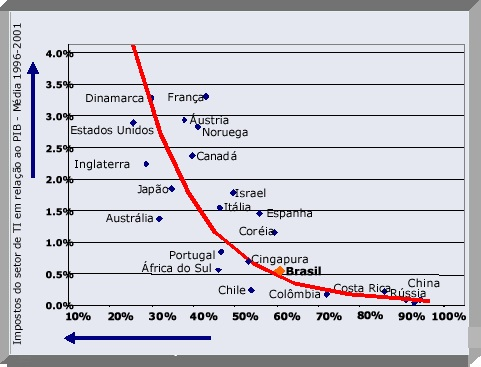
\includegraphics[width=0.5\textwidth]{CIENCIA_DA_COMPUTACAO_Prova2005-utf8_figuras/fig-0033.jpg}
		\caption{Participação de imposto do setor de TI no PIB versus índice de pirataria}
	\end{center}
\end{figure}

\begin{figure}[H]
	\begin{center}
		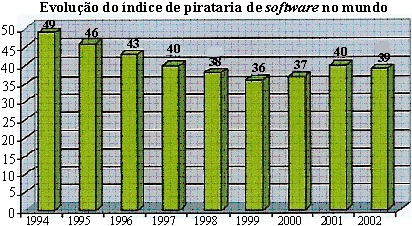
\includegraphics[width=0.5\textwidth]{CIENCIA_DA_COMPUTACAO_Prova2005-utf8_figuras/fig-0031.jpg}
	\end{center}
\end{figure}

\begin{figure}[H]
	\begin{center}
		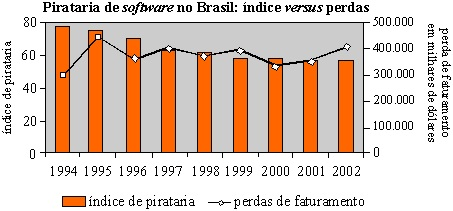
\includegraphics[width=0.5\textwidth]{CIENCIA_DA_COMPUTACAO_Prova2005-utf8_figuras/fig-0032.jpg}
	\end{center}
\end{figure}
Informações obtidas no Relatório Oficial da ABES e BSA, 2005.

A redução da pirataria de software no Brasil e no mundo
é resultado de esforços advindos da iniciativa privada e das
entidades representativas do setor. Um estudo objetivando
mensurar o índice de pirataria no mundo e os benefícios de sua
redução apresentou os gráficos acima, obtidos de uma amostra
de 57 países, incluindo-se o Brasil.
Com base nas informações apresentadas, é correto afirmar que
I a taxa de redução do índice de pirataria de software no mundo
manteve-se constante ano após ano no período mostrado.
II o Brasil reduziu em torno de 25% seu índice de pirataria de
software, comparando os anos de 1994 e 2002.
III o Brasil foi, entre os países mostrados, o que apresentou a maior
redução do índice de pirataria no período estudado.
IV países com maior participação do setor de TI no PIB apresentam,
normalmente, menores índices de pirataria.
V o Brasil apresentou aumento de faturamento no período de 2000
a 2002, apesar do aumento de pirataria.
Estão certos apenas os itens
	\begin{enumerate}[label=\alph*)]
		\item  I e II. 
		\item  I e III. 
		\item  II e IV.
		\item  III e V.
		\item  IV e V.
	\end{enumerate}

\question (\textbf{Enade} $|$ \textbf{CC}-\textbf{2005} $|$ \textbf{Objetiva})
Suponha que uma empresa esteja projetando um protocolo de
transporte orientado a conexão. Suponha, ainda, que os projetistas
tenham pouca experiência e que alguns requisitos originalmente
listados não sejam típicos de um protocolo de transporte
orientado a conexão. A seguir, apresenta-se a lista dos
requisitos propostos pela equipe de projetistas.
I O protocolo deve controlar a transmissão por meio de
mecanismo de janela deslizante (sliding window). Vários
pacotes poderão ser enviados antes de a origem aguardar uma
confirmação de recepção. O número máximo de pacotes
transmitidos antes de uma confirmação ser recebida será
variável, o que possibilitará o controle do fluxo dos dados.
II O protocolo deve rotear os pacotes entre redes interligadas.
O roteamento deve ser realizado a partir das informações em
tabelas de roteamento. Em uma tabela de roteamento, cada
entrada deve conter o endereço de um destino e o endereço da
próxima máquina para a qual os pacotes devem ser enviados,
de modo a serem encaminhados para o destino.
III Uma comunicação passará por três fases: estabelecimento da
conexão, transferência dos dados e término da conexão. O
protocolo manterá informações sobre uma conexão em uma
estrutura de dados. Uma instância dessa estrutura será alocada
quando uma conexão for estabelecida e será liberada quando
a conexão for terminada.
IV O protocolo deve calcular dinamicamente o tempo (timeout)
que a origem de um pacote deve aguardar até retransmitir a
informação caso a recepção não seja confirmada,
possibilitando que atrasos variáveis sejam acomodados. Isso
deverá ser feito por meio de um algoritmo de retransmissão
adaptativo que periodicamente ajuste o timeout.
Para um protocolo de transporte orientado a conexão, são
adequados apenas os requisitos
	\begin{enumerate}[label=\alph*)]
		\item  I e II.
		\item  I e IV.
		\item  II e III.
		\item  I, III e IV.
		\item  II, III e IV.
	\end{enumerate}

\question (\textbf{Enade} $|$ \textbf{CC}-\textbf{2005} $|$ \textbf{Objetiva})


\begin{figure}[H]
	\begin{center}
		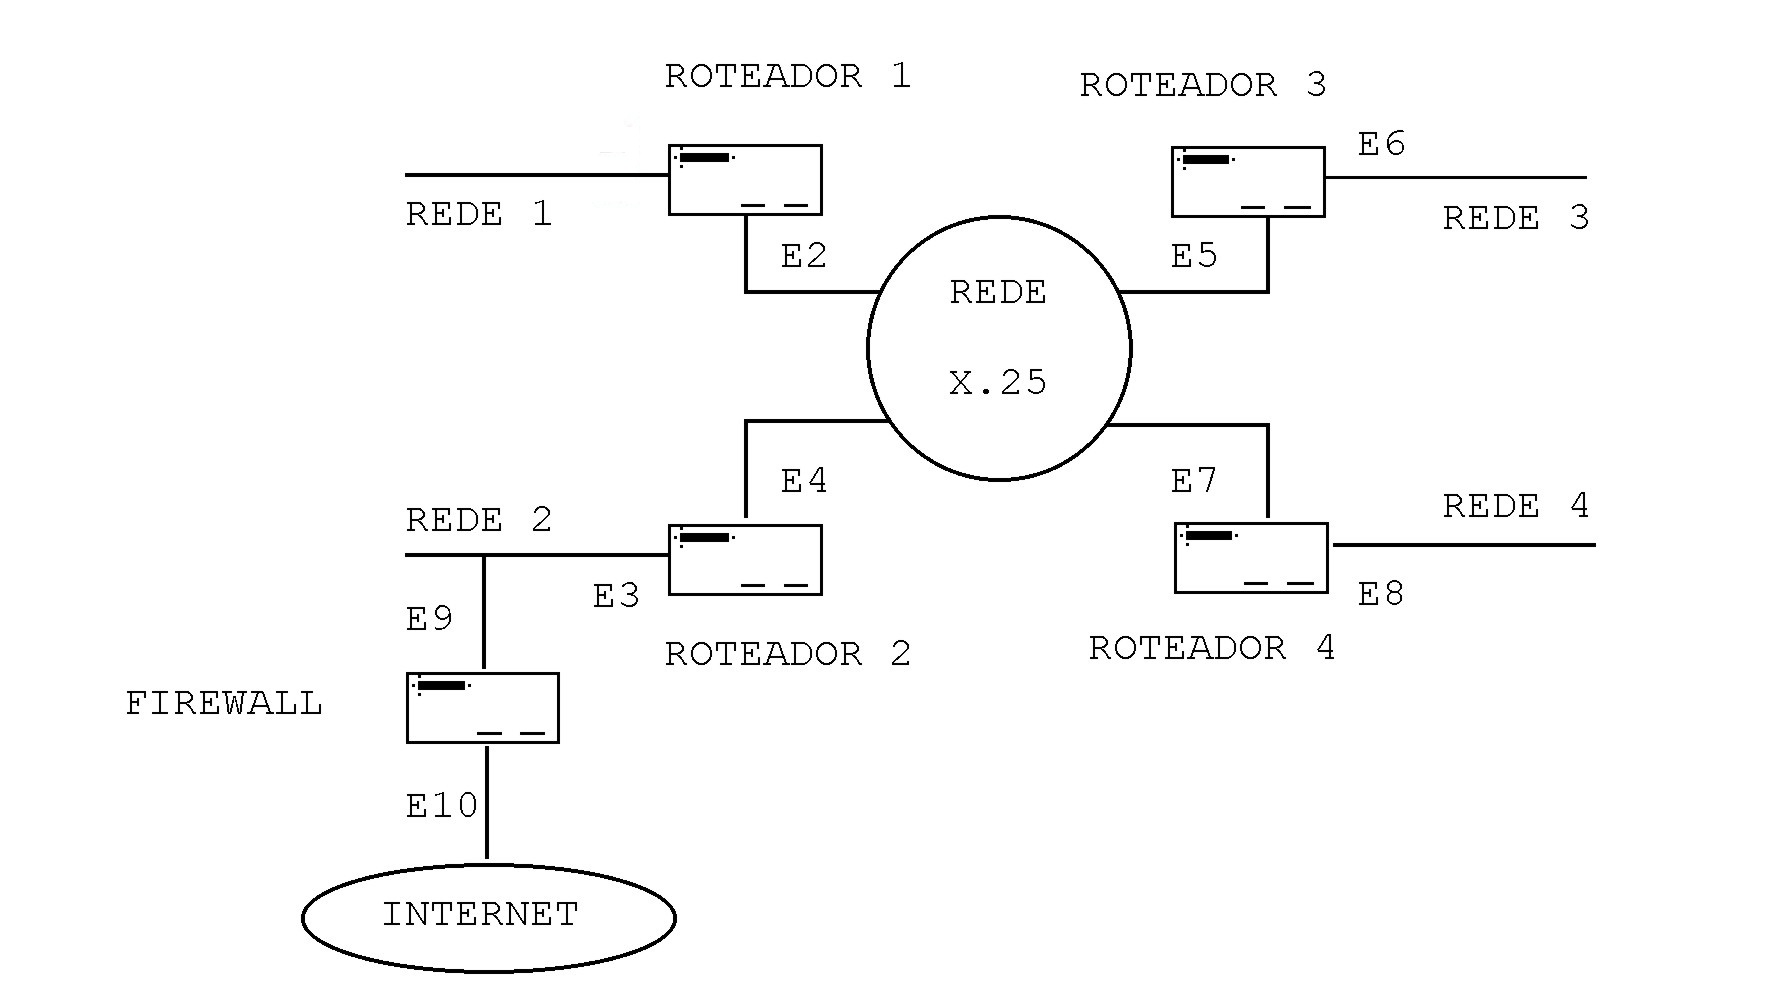
\includegraphics[width=0.5\textwidth]{CIENCIA_DA_COMPUTACAO_Prova2005-utf8_figuras/fig-0034.jpg}
	\end{center}
\end{figure}

A rede de uma empresa cujo esquema está ilustrado
acima é composta por 4 redes TCP/IP locais. Essas redes
TCP/IP são interligadas por uma rede X.25, que opera
como túnel para as 4 redes. As placas dos computadores
pertencentes a essas redes são numeradas com endereços IP
das redes 10.0.0.0 ou 164.41.0.0. Um firewall protege a
rede no acesso à Internet, sendo que, a partir de qualquer
máquina na rede, pode-se acessar a Internet.
A partir dessas informações, julgue os itens a seguir, relativos à
rede da referida empresa, considerando o seu correto
funcionamento.
I É correto utilizar a máscara 255.255.0.0 para segmentar a
rede.
II Os endereços de E1 a E9 podem ser endereços na rede
10.0.0.0.
III Os endereços E2, E4, E5 e E7 devem estar em uma mesma
sub-rede.
IV O endereço E10 deve ser um endereço na rede 164.41.0.0.
V O firewall deve traduzir entre os endereços na rede 10.0.0.0
e os endereços na rede 164.41.0.0.
VI Os pacotes X.25 são transferidos dentro de pacotes IP.
VII Não devem ter sido atribuídos endereços X.25 aos
roteadores 1, 2, 3 e 4.
VIII A rota default nas tabelas de roteamento dos roteadores
1, 3 e 4 é o endereço E4.
IX A rota default na tabela de roteamento do roteador 2 é o
endereço E10.
X Os endereços na rede 10.0.0.0 são visíveis pelas máquinas
que estiverem na Internet.
Estão certos apenas os itens
	\begin{enumerate}[label=\alph*)]
		\item  I, II, III, V, VIII e X.
		\item  I, II, III, IV, V e VIII.
		\item  II, IV, V, VIII, IX e X.
		\item  III, V, VI, VII, VIII e IX.
		\item  III, IV, V, VII, VIII e IX.
	\end{enumerate}

\question (\textbf{Enade} $|$ \textbf{CC}-\textbf{2005} $|$ \textbf{Dissertativa})

\begin{figure}[H]
	\begin{center}
		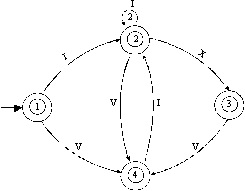
\includegraphics[width=0.5\textwidth]{CIENCIA_DA_COMPUTACAO_Prova2005-utf8_figuras/fig-0040.jpg}
	\end{center}
\end{figure}

A máquina finita de estados (MFE) cujo diagrama é visto ao lado
reconhece seqüências de caracteres compostos pelas letras I, V e X, que
representam, em notação romana, números correspondentes ao intervalo de
1 a 9, na notação arábica. Considere que todas as sentenças de entrada da
MFE representam números romanos válidos, ou seja, a MFE não tem
mecanismo de tratamento de erros. Observe a correspondência da
representação dos alfabetos romano e arábito fornecida pela tabela abaixo.
alfabeto Notação:
romano arábico 
  
\begin{figure}[H]
	\begin{center}
		
\includegraphics[width=0.5\textwidth]{CIENCIA_DA_COMPUTACAO_Prova2005-utf8_figuras/fig-0035.jpg}
	\end{center}
\end{figure}

\begin{figure}[H]
	\begin{center}
		
\includegraphics[width=0.5\textwidth]{CIENCIA_DA_COMPUTACAO_Prova2005-utf8_figuras/fig-0036.jpg}
	\end{center}
\end{figure}
estado inicial
 
\begin{figure}[H]
	\begin{center}
		
\includegraphics[width=0.5\textwidth]{CIENCIA_DA_COMPUTACAO_Prova2005-utf8_figuras/fig-0037.jpg}
		\caption{estado final j}
	\end{center}
\end{figure}
 
\begin{figure}[H]
	\begin{center}
		
\includegraphics[width=0.5\textwidth]{CIENCIA_DA_COMPUTACAO_Prova2005-utf8_figuras/fig-0038.jpg}
		\caption{n é o número máximo de transições possíveis no respectivo estado}
	\end{center}
\end{figure}

\begin{figure}[H]
	\begin{center}
		
\includegraphics[width=0.5\textwidth]{CIENCIA_DA_COMPUTACAO_Prova2005-utf8_figuras/fig-0039.jpg}
	\end{center}
\end{figure}
transição após reconhecimento do caractere "
I 1
V 5
X 10
L 50
C 100
D 500
Considerando essas informações, estenda a MFE apresentada acima para:
a) reconhecer números no alfabeto romano correspondentes aos números de 1 a 20 no alfabeto arábico, com no máximo oito estados.
(valor: 5,0 pontos)
RASCUNHO
b) reconhecer números no alfabeto romano correspondentes aos números de 1 a 500 no alfabeto arábico, com no máximo oito
estados. (valor: 5,0 pontos)
RASCUNHO

As questões de 71 a 85, a seguir, são específicas para os estudantes de cursos com perfil profissional de
ENGENHARIA DE COMPUTAÇÃO
\question (\textbf{Enade} $|$ \textbf{CC}-\textbf{2005} $|$ \textbf{Objetiva})
Sistemas operacionais de tempo real são utilizados em controle
de processos automatizados, em que o tempo de resposta a
determinados eventos é um fator crítico. Com relação a esse
assunto, julgue os itens seguintes.
I Sistemas de tempo real estritos (hard real-time) não utilizam
dispositivos de memória secundária (como discos), pois estes
não oferecem garantia de término das operações dentro de
uma quantidade máxima de tempo.
II Um sistema operacional de propósito geral pode ser
modificado para ser de tempo real atribuindo-se prioridades
fixas para cada um dos processos.
III O escalonamento mais utilizado por sistemas operacionais de
tempo real é o shortest-job-first (tarefa mais curta primeiro).
Assinale a opção correta.
	\begin{enumerate}[label=\alph*)]
		\item  Apenas um item está certo.
		\item  Apenas os itens I e II estão certos.
		\item  Apenas os itens I e III estão certos.
		\item  Apenas os itens II e III estão certos.
		\item  Todos os itens estão certos.
	\end{enumerate}

\question (\textbf{Enade} $|$ \textbf{CC}-\textbf{2005} $|$ \textbf{Objetiva})
1 2 3
T T T
1
2
3
4
5
6
7
8
bloqueia A
recupera A
atualiza A
desbloqueia A
bloqueia B
recupera B
atualiza B
desbloqueia B
bloqueia B
recupera B
atualiza B
bloqueia A
recupera A
atualiza A
desbloqueia A
desbloqueia B
bloqueia B
recupera B
atualiza B
bloqueia A
recupera A
desbloqueia A
desbloqueia B
i j
A execução de duas transações, T e T , em um banco de dados,
é serializável se produz o mesmo resultado para a execução serial
de qualquer intercalação de operações dessas transações
i j j i
(T seguida de T ou T seguida de T ). O uso de bloqueios (locks)
é uma maneira de se garantir que transações concorrentes sejam
serializáveis. A tabela acima mostra informações relativas a três
1 2 3
transações, T , T e T , que operam sobre dois dados
compartilhados, A e B, e utilizam bloqueios para controle de
1 2 3
concorrência. Com relação às transações T , T e T , julgue os
itens seguintes.
1 2
I O conjunto (T , T ) não é serializável, e há o perigo de
ocorrer deadlock durante a execução concorrente dessas
transações.
1 3
II O conjunto (T , T ) não é serializável, mas não há o perigo de
ocorrer deadlock durante a execução concorrente dessas
transações.
2 3
III O conjunto (T , T ) é serializável, e não há o perigo de
ocorrer deadlock durante a execução concorrente dessas
transações.
Assinale a opção correta.
	\begin{enumerate}[label=\alph*)]
		\item  Apenas um item está certo.
		\item  Apenas os itens I e II estão certos.
		\item  Apenas os itens I e III estão certos.
		\item  Apenas os itens II e III estão certos.
		\item  Todos os itens estão certos.
	\end{enumerate}

\question (\textbf{Enade} $|$ \textbf{CC}-\textbf{2005} $|$ \textbf{Objetiva})
Considere o seguinte script SQL de criação de um banco de
dados.
\begin{minted}{sql}
CREATE TABLE PECAS (CODIGO NUMERIC(5) NOT NULL,
DESCRICAO VARCHAR(20) NOT NULL,
ESTOQUE NUMERIC(5) NOT NULL,
PRIMARY KEY(CODIGO));
CREATE TABLE FORNECEDORES
(COD_FORN NUMERIC(3) NOT NULL,
NOME VARCHAR(30) NOT NULL,
PRIMARY KEY(COD_FORN));
CREATE TABLE FORNECIMENTOS
(COD_PECA NUMERIC(5) NOT NULL,
COD_FORN NUMERIC(3) NOT NULL,
QUANTIDADE NUMERIC(4) NOT NULL,
PRIMARY KEY(COD_PECA, COD_FORN),
FOREIGN KEY (COD_PECA) REFERENCES PECAS,
FOREIGN KEY (COD_FORN) REFERENCES
FORNECEDORES);
\end{minted} 
A partir desse script, assinale a opção que apresenta comando
SQL que permite obter uma lista que contenha o nome de cada
fornecedor que tenha fornecido alguma peça, o código da peça
fornecida, a descrição dessa peça e a quantidade fornecida da
referida peça.
	\begin{enumerate}[label=\alph*)]
		\item  SELECT * FROM PECAS, FORNECEDORES,
FORNECIMENTOS;
		\item  SELECT * FROM PECAS, FORNECEDORES,
FORNECIMENTOS WHERE PECAS.CODIGO =
FORNECIMENTOS.COD\_PECA AND
FORNECEDORES.COD\_FORN =
FORNECIMENTOS.COD\_FORN;
		\item  SELECT NOME, CODIGO, DESCRICAO, QUANTIDADE
FROM PECAS, FORNECEDORES, FORNECIMENTOS;
		\item  SELECT NOME, CODIGO, DESCRICAO, QUANTIDADE
FROM PECAS, FORNECEDORES, FORNECIMENTOS
WHERE PECAS.CODIGO = FORNECIMENTOS.COD\_PECA
AND FORNECEDORES.COD\_FORN =
FORNECIMENTOS.COD\_FORN;
		\item  SELECT DISTINCT NOME, CODIGO, DESCRICAO,
QUANTIDADE
FROM PECAS, FORNECEDORES, FORNECIMENTOS
WHERE CODIGO = COD\_PECA;
	\end{enumerate}

\question (\textbf{Enade} $|$ \textbf{CC}-\textbf{2005} $|$ \textbf{Objetiva})
No que diz respeito às redes neurais, assinale a opção correta.
	\begin{enumerate}[label=\alph*)]
		\item  O treinamento de uma rede neural tem tempo determinado de
execução.
		\item  Não há problemas em realizar o teste de desempenho de uma
rede neural com o mesmo conjunto de dados usado para o
treinamento.
		\item  O número de pesos de uma rede neural não influencia a
rapidez com que ela processa dados.
		\item  O aprendizado supervisionado é o paradigma de treinamento
mais utilizado para desenvolver aplicações de redes neurais
para classificação e predição.
		\item  O número de camadas ocultas de uma rede de alimentação
direta é inversamente proporcional ao aumento do espaço de
hipóteses que ela pode representar.
	\end{enumerate}

\question (\textbf{Enade} $|$ \textbf{CC}-\textbf{2005} $|$ \textbf{Objetiva})
Um engenheiro de uma companhia fabricante de
memórias semicondutoras estudou o comportamento
do custo em função do número de bits da fabricação de
um chip de memória RAM com determinada
tecnologia. Ele chegou à conclusão de que,
considerando-se a evolução tecnológica, o custo C(x),
expresso em determinada unidade monetária, de um
chip de memória RAM com x bits, na data de conclusão
do processo de fabricação, seria determinado pela
equação
Considerando-se que o modelo desenvolvido pelo engenheiro
esteja correto, caso a empresa decida pelo chip de menor
custo, ela deverá optar por um chip com memória de
capacidade de
	\begin{enumerate}[label=\alph*)]
		\item  256 megabits.
		\item  512 megabits.
		\item  1.024 megabits.
		\item  2.048 megabits.
		\item  4.096 megabits.
	\end{enumerate}

\question (\textbf{Enade} $|$ \textbf{CC}-\textbf{2005} $|$ \textbf{Objetiva})
O termo imagem designa uma função
intensidade luminosa bidimensional f, em que um valor
de intensidade é associado a coordenadas espaciais
(x, y). Uma imagem digital é obtida pela digitalização
das coordenadas espaciais por meio de um processo
conhecido como amostragem da imagem. Dessa
forma, uma imagem contínua monocromática f(x, y) é
aproximada por amostras igualmente espaçadas,
arranjadas na forma de uma matriz N×M, em que cada
min max
elemento é um valor inteiro g. O intervalo [G , G ],
do menor ao maior valor de intensidade g, é
min
denominado escala de cinza. Normalmente, G = 0
max
corresponde a preto, e G = G corresponde ao
branco.
Considerando os conceitos apresentados acima, assinale a
opção correta.
	\begin{enumerate}[label=\alph*)]
		\item  O processo de digitalização da imagem requer que as
dimensões N e M da matriz mencionada acima sejam
múltiplas do número de tons de cinza na imagem.
		\item  Para imagens binárias, se L for o número de tons de cinza
representáveis, e L = 2 , então k = 2.
k
		\item  Os métodos para realce de imagens que operam no
domínio espacial fazem uso do conceito de vizinhança de
pixel.
		\item  Métodos de filtragem normalmente usam máscaras para
impedir a transformação dos níveis de cinza dos pixels da
imagem.
		\item  Limiarização é um tipo de processamento de imagens que
amplia o número de níveis de cinza da imagem.
	\end{enumerate}

\question (\textbf{Enade} $|$ \textbf{CC}-\textbf{2005} $|$ \textbf{Objetiva})

\begin{figure}[H]
	\begin{center}
		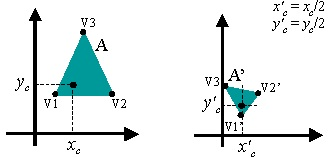
\includegraphics[width=0.5\textwidth]{CIENCIA_DA_COMPUTACAO_Prova2005-utf8_figuras/fig-0041.jpg}
	\end{center}
\end{figure}
Observe a situação representada acima, em que o triângulo
identificado por A sofre transformações geométricas que o levam para
a situação identificada por A’. Considerando-se dx e dy parâmetros
de translação e s, parâmetro fator de escala, então o triângulo A’ pode
ser obtido a partir da aplicação da seguinte seqüência de
transformações aos vértices do triângulo A:
c c
	\begin{enumerate}[label=\alph*)]
		\item  rotação em torno do ponto (x , y ); escala com fator uniforme
s = 2.
c c
		\item  rotação em torno do ponto (x , y ); escala com fator uniforme
s = 0,5.
c c
		\item  rotação em torno do ponto (x' , y' ); escala com fator
uniforme s = 0,5; translação com parâmetros de deslocamento
c c
dx = !x e dy = !y .
		\item  escala com fator uniforme s = 0,5; translação com parâmetros de
c c
deslocamento dx = x' e dy = y' ; rotação em torno do
c c
ponto (x , y ).
c c
		\item  tanslação com parâmetros de deslocamento dx = !x e dy = !y ;
c c
rotação em torno do ponto (x , y ); translação com parâmetros
c c
de deslocamento dx = x e dy = y ; escala com fator uniforme
s = 0,5.
	\end{enumerate}

\question (\textbf{Enade} $|$ \textbf{CC}-\textbf{2005} $|$ \textbf{Objetiva})
Dispositivos Lógicos Programáveis (DLP, ou PLD — programmable
logic devices) são muito utilizados hoje em dia para o projeto de
circuitos digitais especiais. Com relação a esse assunto, julgue os
itens a seguir.
I Como um PLA (programmable logic array) somente implementa
equações booleanas descritas na forma de soma de termos-
produto, e não implementa portas lógicas multinível, então nem
todas as funções booleanas podem ser implementadas em um
PLA.
II Em uma PROM (programmable ROM), o arranjo de portas AND
é fixo, e somente o arranjo de portas OR pode ser programado; em
um PAL (programmable array logic), o arranjo de portas OR é
fixo, e somente o array de portas AND é programável; e, em um
PLA (programmable logic array), tanto o arranjo de portas AND
como o de portas OR são programáveis.
III Um circuito digital implementado por meio de um dispositivo
lógico programável ocupa mais área e consome mais potência do
que um circuito integrado dedicado, mas, em compensação, ele
pode operar em freqüências maiores, pois seus transistores e
portas lógicas são projetados de forma a otimizar o chaveamento
de estados.
Assinale a opção correta.
	\begin{enumerate}[label=\alph*)]
		\item  Apenas o item II está certo.
		\item  Apenas o item III está certo.
		\item  Apenas os itens I e II estão certos.
		\item  Apenas os itens I e III estão certos.
		\item  Apenas os itens II e III estão certos.
	\end{enumerate}

\question (\textbf{Enade} $|$ \textbf{CC}-\textbf{2005} $|$ \textbf{Objetiva})
xpto( [ ], R, R ).
xpto( [H | T1], Y, [H | T2] ) :- xpto( T1, Y, T2 ).
zpto( X, [X|Y] ).
zpto( X, [Y|Z] ) :- zpto( X, Z ).
Com relação aos predicados escritos em Prolog acima, julgue os
itens a seguir.
I A execução de xpto([1,2,3],[ ], F) conclui com sucesso
instanciando F para [1,2,3].
II A execução de zpto(5,[1,2,3] ) conclui sem sucesso.
III A execução de zpto(X,[1,2,3]) conclui com sucesso,
instanciando X para 1.
Assinale a opção correta.
	\begin{enumerate}[label=\alph*)]
		\item  Apenas um item está certo.
		\item  Apenas os itens I e II estão certos.
		\item  Apenas os itens I e III estão certos.
		\item  Apenas os itens II e III estão certos.
		\item  Todos os itens estão certos.
	\end{enumerate}

\question (\textbf{Enade} $|$ \textbf{CC}-\textbf{2005} $|$ \textbf{Objetiva})

\begin{figure}[H]
	\begin{center}
		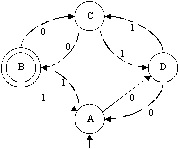
\includegraphics[width=0.5\textwidth]{CIENCIA_DA_COMPUTACAO_Prova2005-utf8_figuras/fig-0042.jpg}
	\end{center}
\end{figure}
Que cadeia é reconhecida pelo
autômato representado pelo
diagrama de estados ao lado?
	\begin{enumerate}[label=\alph*)]
		\item  101010
		\item  111011000
		\item  11111000
		\item  10100
		\item  00110011
	\end{enumerate}

\question (\textbf{Enade} $|$ \textbf{CC}-\textbf{2005} $|$ \textbf{Objetiva})
O estudo de dimensionamento e de desempenho de redes de
comunicação é uma ciência que usa constantemente os resultados da
teoria de filas. Nesse tipo de análise, é comum a adoção de modelos
de filas M/M/1 para a análise de enlaces de roteadores e
comutadores. Nesse tipo de modelo, a chegada de pacotes para
transmissão e a transmissão deles são processos de Poisson. Assim,
as características da fila que se forma em cada enlace podem ser
determinadas em função da taxa de chegada (tempo médio decorrido
entre a chegada de pacotes sucessivos encaminhados para
transmissão pelo enlace) e da taxa de serviço (tempo médio para
transmissão de um pacote). Acerca do modelo M/M/1 aplicado ao
estudo de capacidade e desempenho de enlaces de redes, por
comutação de pacotes, assinale a opção correta.
	\begin{enumerate}[label=\alph*)]
		\item  Caso a taxa de chegada seja maior que a taxa de serviço (taxa de
saída), conclui-se que o enlace está subdimensionado e haverá
perda de pacotes.
		\item  A taxa de serviço é independente do tamanho do pacote.
		\item  Em um roteador com múltiplos enlaces, a taxa de chegada para
cada enlace é igual ao somatório das capacidades de todos os
enlaces dividido pelo número de enlaces do roteador.
		\item  O modelo M/M/1 apresenta instabilidade numérica sempre que
a taxa de chegada for próxima de zero.
		\item  Quando a taxa de chegada é menor que a taxa de serviço,
pode-se esperar que o número médio de pacotes na fila seja igual
a zero.
	\end{enumerate}

\question (\textbf{Enade} $|$ \textbf{CC}-\textbf{2005} $|$ \textbf{Objetiva})

\begin{figure}[H]
	\begin{center}
		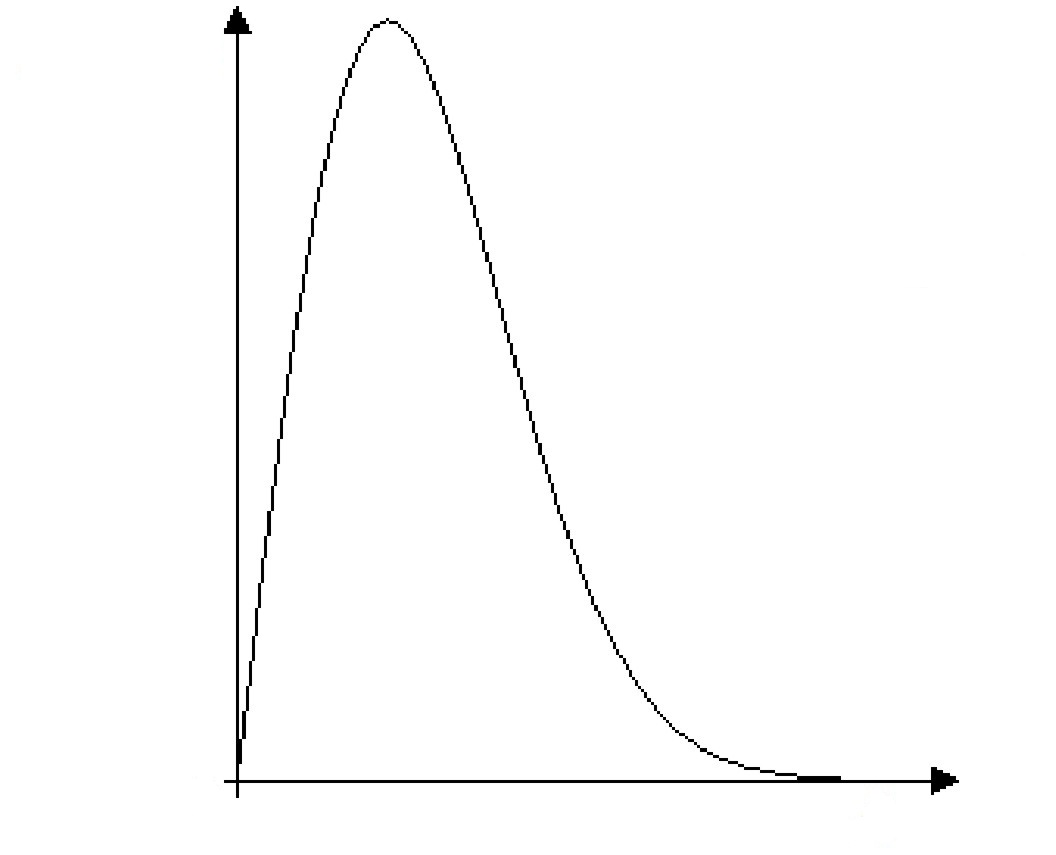
\includegraphics[width=0.5\textwidth]{CIENCIA_DA_COMPUTACAO_Prova2005-utf8_figuras/fig-0043.jpg}
	\end{center}
\end{figure}
Considere que, em uma rede WLAN, a função de
densidade de probabilidade (PDF) de erro de bit na
transmissão entre um computador conectado à rede e o
erro
ponto de acesso (access point) — p (d) — seja dada
pela função cujo gráfico está mostrado acima, em que d
\$ 0 é a distância entre o ponto de acesso e o
computador.
Considerando essas informações, julgue os itens a seguir.
I A probabilidade de erro de bit na transmissão no caso de o
0
computador estar localizado à distância d é dada
por .
II Sabendo-se que a média da distribuição correspondente
à PDF acima mencionada é igual a x, conclui-se que é de
0,5 a probabilidade de erro de bit na transmissão no caso
de o computador estar localizado à distância d = x.
III Supondo-se que o sistema de transmissão seja binário, as
informações apresentadas são suficientes para se
concluir que a probabilidade de erro dado que foi enviado
um bit 1 é igual à probabilidade de erro dado que foi
enviado um bit 0.
Assinale a opção correta.
	\begin{enumerate}[label=\alph*)]
		\item  Apenas um item está certo.
		\item  Apenas os itens I e II estão certos.
		\item  Apenas os itens I e III estão certos.
		\item  Apenas os itens II e III estão certos.
		\item  Todos os itens estão certos.
	\end{enumerate}

\question (\textbf{Enade} $|$ \textbf{CC}-\textbf{2005} $|$ \textbf{Objetiva})
Com relação à tecnologia bluetooth, que possibilita a
comunicação sem fios entre dispositivos, assinale a opção
correta.
	\begin{enumerate}[label=\alph*)]
		\item  Essa tecnologia utiliza a transmissão em enlace via rádio na
banda de freqüência VHF.
		\item  Essa tecnologia possibilita a transmissão de voz e dados a
curtas distâncias.
		\item  Um dispositivo pode assumir, simultaneamente, o papel de
mestre e de escravo em uma mesma piconet que utiliza essa
tecnologia.
		\item  Uma piconet pode ser formada por até 255 mestres e
255 escravos.
		\item  Um dispositivo pode participar, simultaneamente, de duas
piconets, desde que ele seja mestre em ambas.
	\end{enumerate}

\question (\textbf{Enade} $|$ \textbf{CC}-\textbf{2005} $|$ \textbf{Objetiva})
Considere que uma empresa esteja projetando um protocolo da camada de rede. Considere, ainda, que a equipe de projeto tenha
proposto o seguinte conjunto de requisitos.
I O protocolo deve prover um serviço de comunicação não-orientado a conexão e sem garantia da entrega. O protocolo não é
responsável por ordenar os datagramas que, embora recebidos com sucesso, estejam fora da ordem em que foram transmitidos.
II Os datagramas devem conter, além dos endereços de rede das máquinas, números que identifiquem as entidades nas máquinas de
origem e destino para distinguirem as entidades nas máquinas envolvidas em uma comunicação.
III O protocolo deve evitar que as aplicações tenham de definir os formatos usados para representar os dados nas máquinas. Na
transmissão, o protocolo deve converter os dados de um formato específico de máquina para um formato independente de máquina.
Na recepção, deve converter de um formato independente de máquina para um formato específico de máquina.
IV O protocolo poderá fragmentar um datagrama na origem e remontá-lo no destino, para que dados sejam transmitidos por meio de
redes cujas camadas físicas tenham tamanhos variados para as unidades máximas de transferência (maximum transfer unit).
V O protocolo deve implementar o controle de acesso ao meio de transmissão. Antes de transmitir, deve aguardar o meio de
transmissão ficar livre. Se outras máquinas tentarem transmitir ao mesmo tempo, ele deve enviar um sinal para garantir que as
máquinas detectem a colisão. Em seguida, deve aguardar e novamente tentar transmitir.
Entre os requisitos propostos pela equipe de projeto, estão adequados para um um protocolo da camada de rede os requisitos
	\begin{enumerate}[label=\alph*)]
		\item  I, II e IV. 
		\item  I, III e V. 
		\item  I, IV e V. 
		\item  II, III e IV. 
		\item  II, IV e V.
	\end{enumerate}

\question (\textbf{Enade} $|$ \textbf{CC}-\textbf{2005} $|$ \textbf{Dissertativa})
Em sistemas distribuídos, é necessário, muitas vezes, resolver problemas decorrentes do fato de diferentes plataformas
poderem adotar diferentes formas para representar os dados.
A respeito de sistemas distribuídos heterogêneos, faça o que se pede a seguir.
a) Apresente exemplos das diferenças nas formas de representação dos dados que podem causar problemas em sistemas distribuídos.
(valor: 5,0 pontos)
b) Explique o que é eXternal Data Representation (XDR) e como uma biblioteca XDR pode ser usada em chamadas a procedimentos
remotos. (valor: 5,0 pontos)
item a) RASCUNHO
1
2
3
4
5
6
7
8
9
10
item b) RASCUNHO
1
2
3
4
5
6
7
8
9
10
QUESTIONÁRIO DE PERCEPÇÃO SOBRE A PROVA
As questões a seguir visam obter a sua opinião a respeito da qualidade e da adequação da prova que você acabou
de realizar. Escolha, em cada uma delas, a opção que melhor reflete a sua opinião. Use os espaços reservados na folha
de respostas para as suas marcações.
Agradecemos a sua colaboração.
\question (\textbf{Enade} $|$ \textbf{CC}-\textbf{2005} $|$ \textbf{Objetiva})
formação geral?
	\begin{enumerate}[label=\alph*)]
		\item  Muito fácil.
		\item  Fácil.
		\item  Médio.
		\item  Difícil.
		\item  Muito difícil.
	\end{enumerate}

\question (\textbf{Enade} $|$ \textbf{CC}-\textbf{2005} $|$ \textbf{Objetiva})
formação específica?
	\begin{enumerate}[label=\alph*)]
		\item  Muito fácil.
		\item  Fácil.
		\item  Médio.
		\item  Difícil.
		\item  Muito difícil.
	\end{enumerate}

\question (\textbf{Enade} $|$ \textbf{CC}-\textbf{2005} $|$ \textbf{Objetiva})
resolução, como você considera a prova?
	\begin{enumerate}[label=\alph*)]
		\item  Muito longa.
		\item  Longa.
		\item  Adequada.
		\item  Curta.
		\item  Muito curta.
	\end{enumerate}

\question (\textbf{Enade} $|$ \textbf{CC}-\textbf{2005} $|$ \textbf{Objetiva})
formação geral estavam claros e objetivos?
	\begin{enumerate}[label=\alph*)]
		\item  Sim, todos.
		\item  Sim, a maioria.
		\item  Apenas cerca da metade.
		\item  Poucos.
		\item  Não, nenhum.
	\end{enumerate}

\question (\textbf{Enade} $|$ \textbf{CC}-\textbf{2005} $|$ \textbf{Objetiva})
formação específica estavam claros e objetivos?
	\begin{enumerate}[label=\alph*)]
		\item  Sim, todos.
		\item  Sim, a maioria.
		\item  Apenas cerca da metade.
		\item  Poucos.
		\item  Não, nenhum.
	\end{enumerate}

\question (\textbf{Enade} $|$ \textbf{CC}-\textbf{2005} $|$ \textbf{Objetiva})
das questões foram suficientes para resolvê-las?
	\begin{enumerate}[label=\alph*)]
		\item  Sim, até excessivamente.
		\item  Sim, em todas elas.
		\item  Sim, na maioria delas.
		\item  Sim, somente em algumas.
		\item  Não, em nenhuma delas.
	\end{enumerate}

\question (\textbf{Enade} $|$ \textbf{CC}-\textbf{2005} $|$ \textbf{Objetiva})
responder a prova?
	\begin{enumerate}[label=\alph*)]
		\item  Desconhecimento do conteúdo.
		\item  Forma diferente de abordagem do conteúdo.
		\item  Espaço insuficiente para responder às questões.
		\item  Falta de motivação para fazer a prova.
		\item  Não tive dificuldade para responder à prova.
	\end{enumerate}

\question (\textbf{Enade} $|$ \textbf{CC}-\textbf{2005} $|$ \textbf{Objetiva})
você percebeu que
	\begin{enumerate}[label=\alph*)]
		\item  não estudou ainda a maioria dos conteúdos avaliados.
		\item  estudou apenas alguns dos conteúdos avaliados, mas não
os aprendeu.
		\item  estudou a maioria dos conteúdos avaliados, mas não os
aprendeu.
		\item  estudou e aprendeu muitos dos conteúdos avaliados.
		\item  estudou e aprendeu todos os conteúdos avaliados.
	\end{enumerate}

\question (\textbf{Enade} $|$ \textbf{CC}-\textbf{2005} $|$ \textbf{Objetiva}	\begin{enumerate}[label=\alph*)]
		\item  Menos de uma hora.
		\item  Entre uma e duas horas.
		\item  Entre duas e três horas.
		\item  Entre três e quatro horas.
		\item  Usei as quatro horas e não consegui terminar.
	\end{enumerate}

\end{questions}

\end{document}
